\section{Система с запаздыванием}
\subsection{Система 1}
Рассмотрим систему, заданную передаточной функцией: 
\begin{equation}
    W_1(s) = \frac{9s + 2}{s^2 + 6s + 1}e^{-\tau s}
\end{equation}
Разомкнутая система умеет два устойчивых полюса: 
\begin{equation}
    s_{1,2} = -3 \pm 2\sqrt{2}
\end{equation}
Построим годограф Найквиста для системы при различных значениях $\tau$ (рис. \ref{fig:task6_niquist}).
\begin{figure}[ht!]
   \begin{subfigure}[b]{0.5\textwidth}
       \centering
       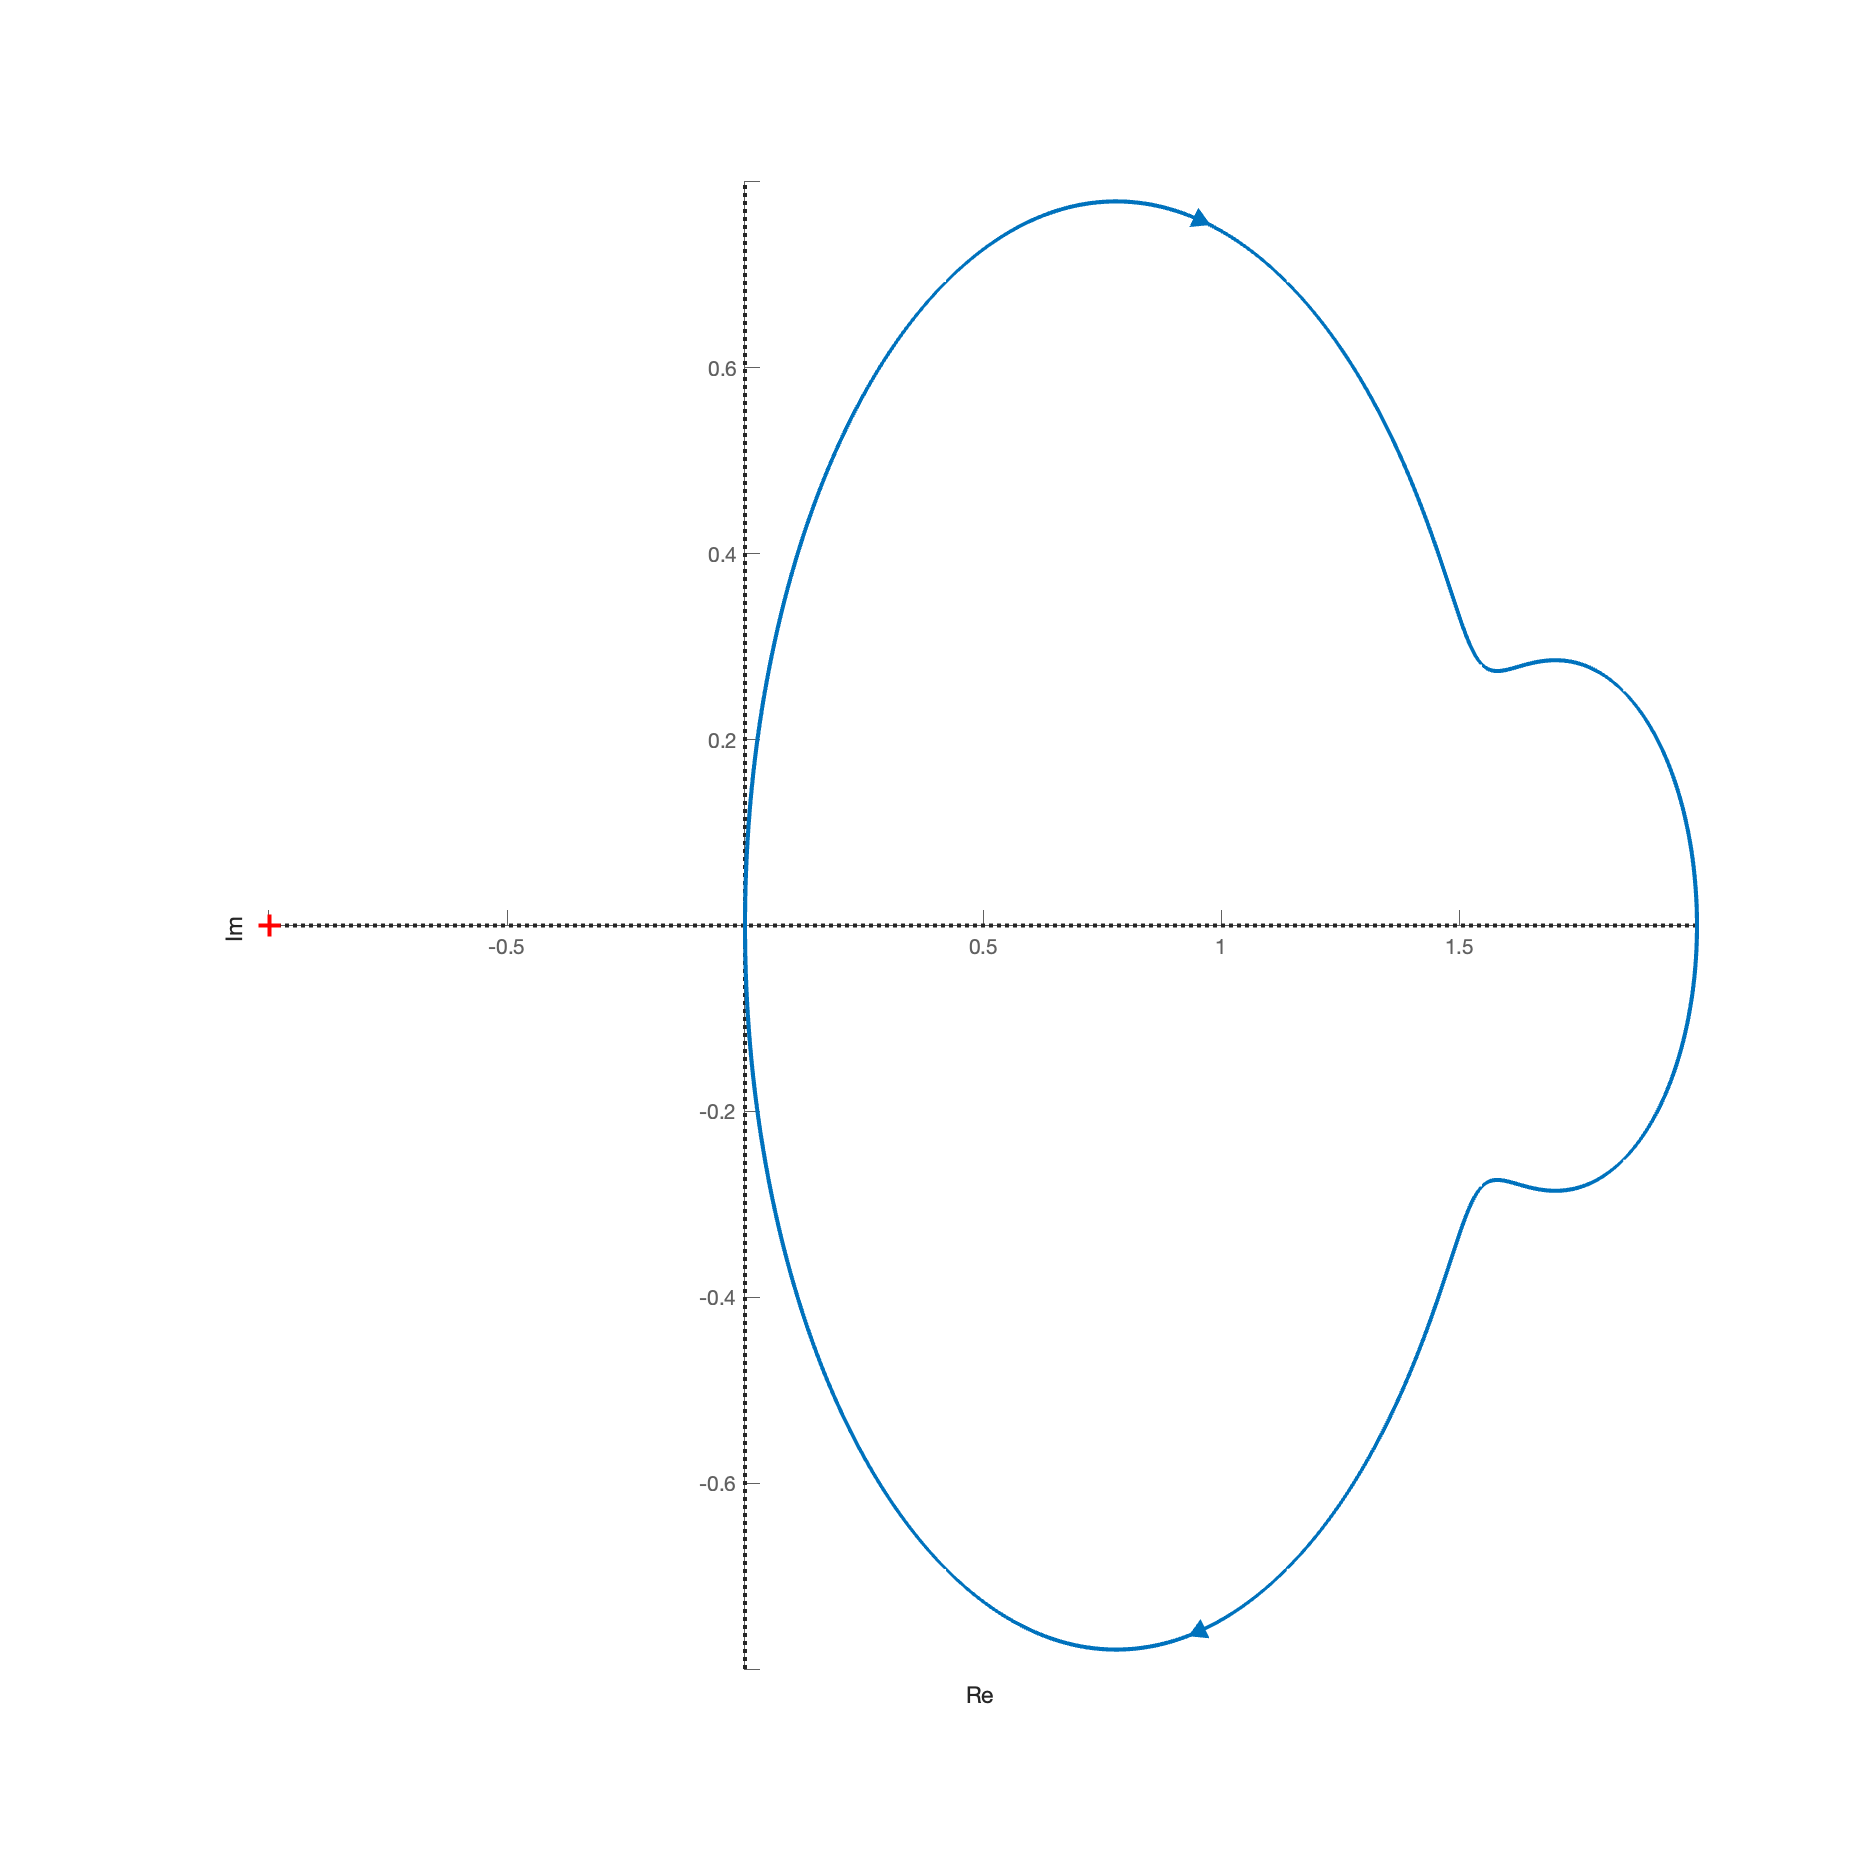
\includegraphics[width=\textwidth]{media/plots/task6_nyquist_open_1.png}
       \caption{$\tau = 0$}
   \end{subfigure}
    \begin{subfigure}[b]{0.5\textwidth}
         \centering
         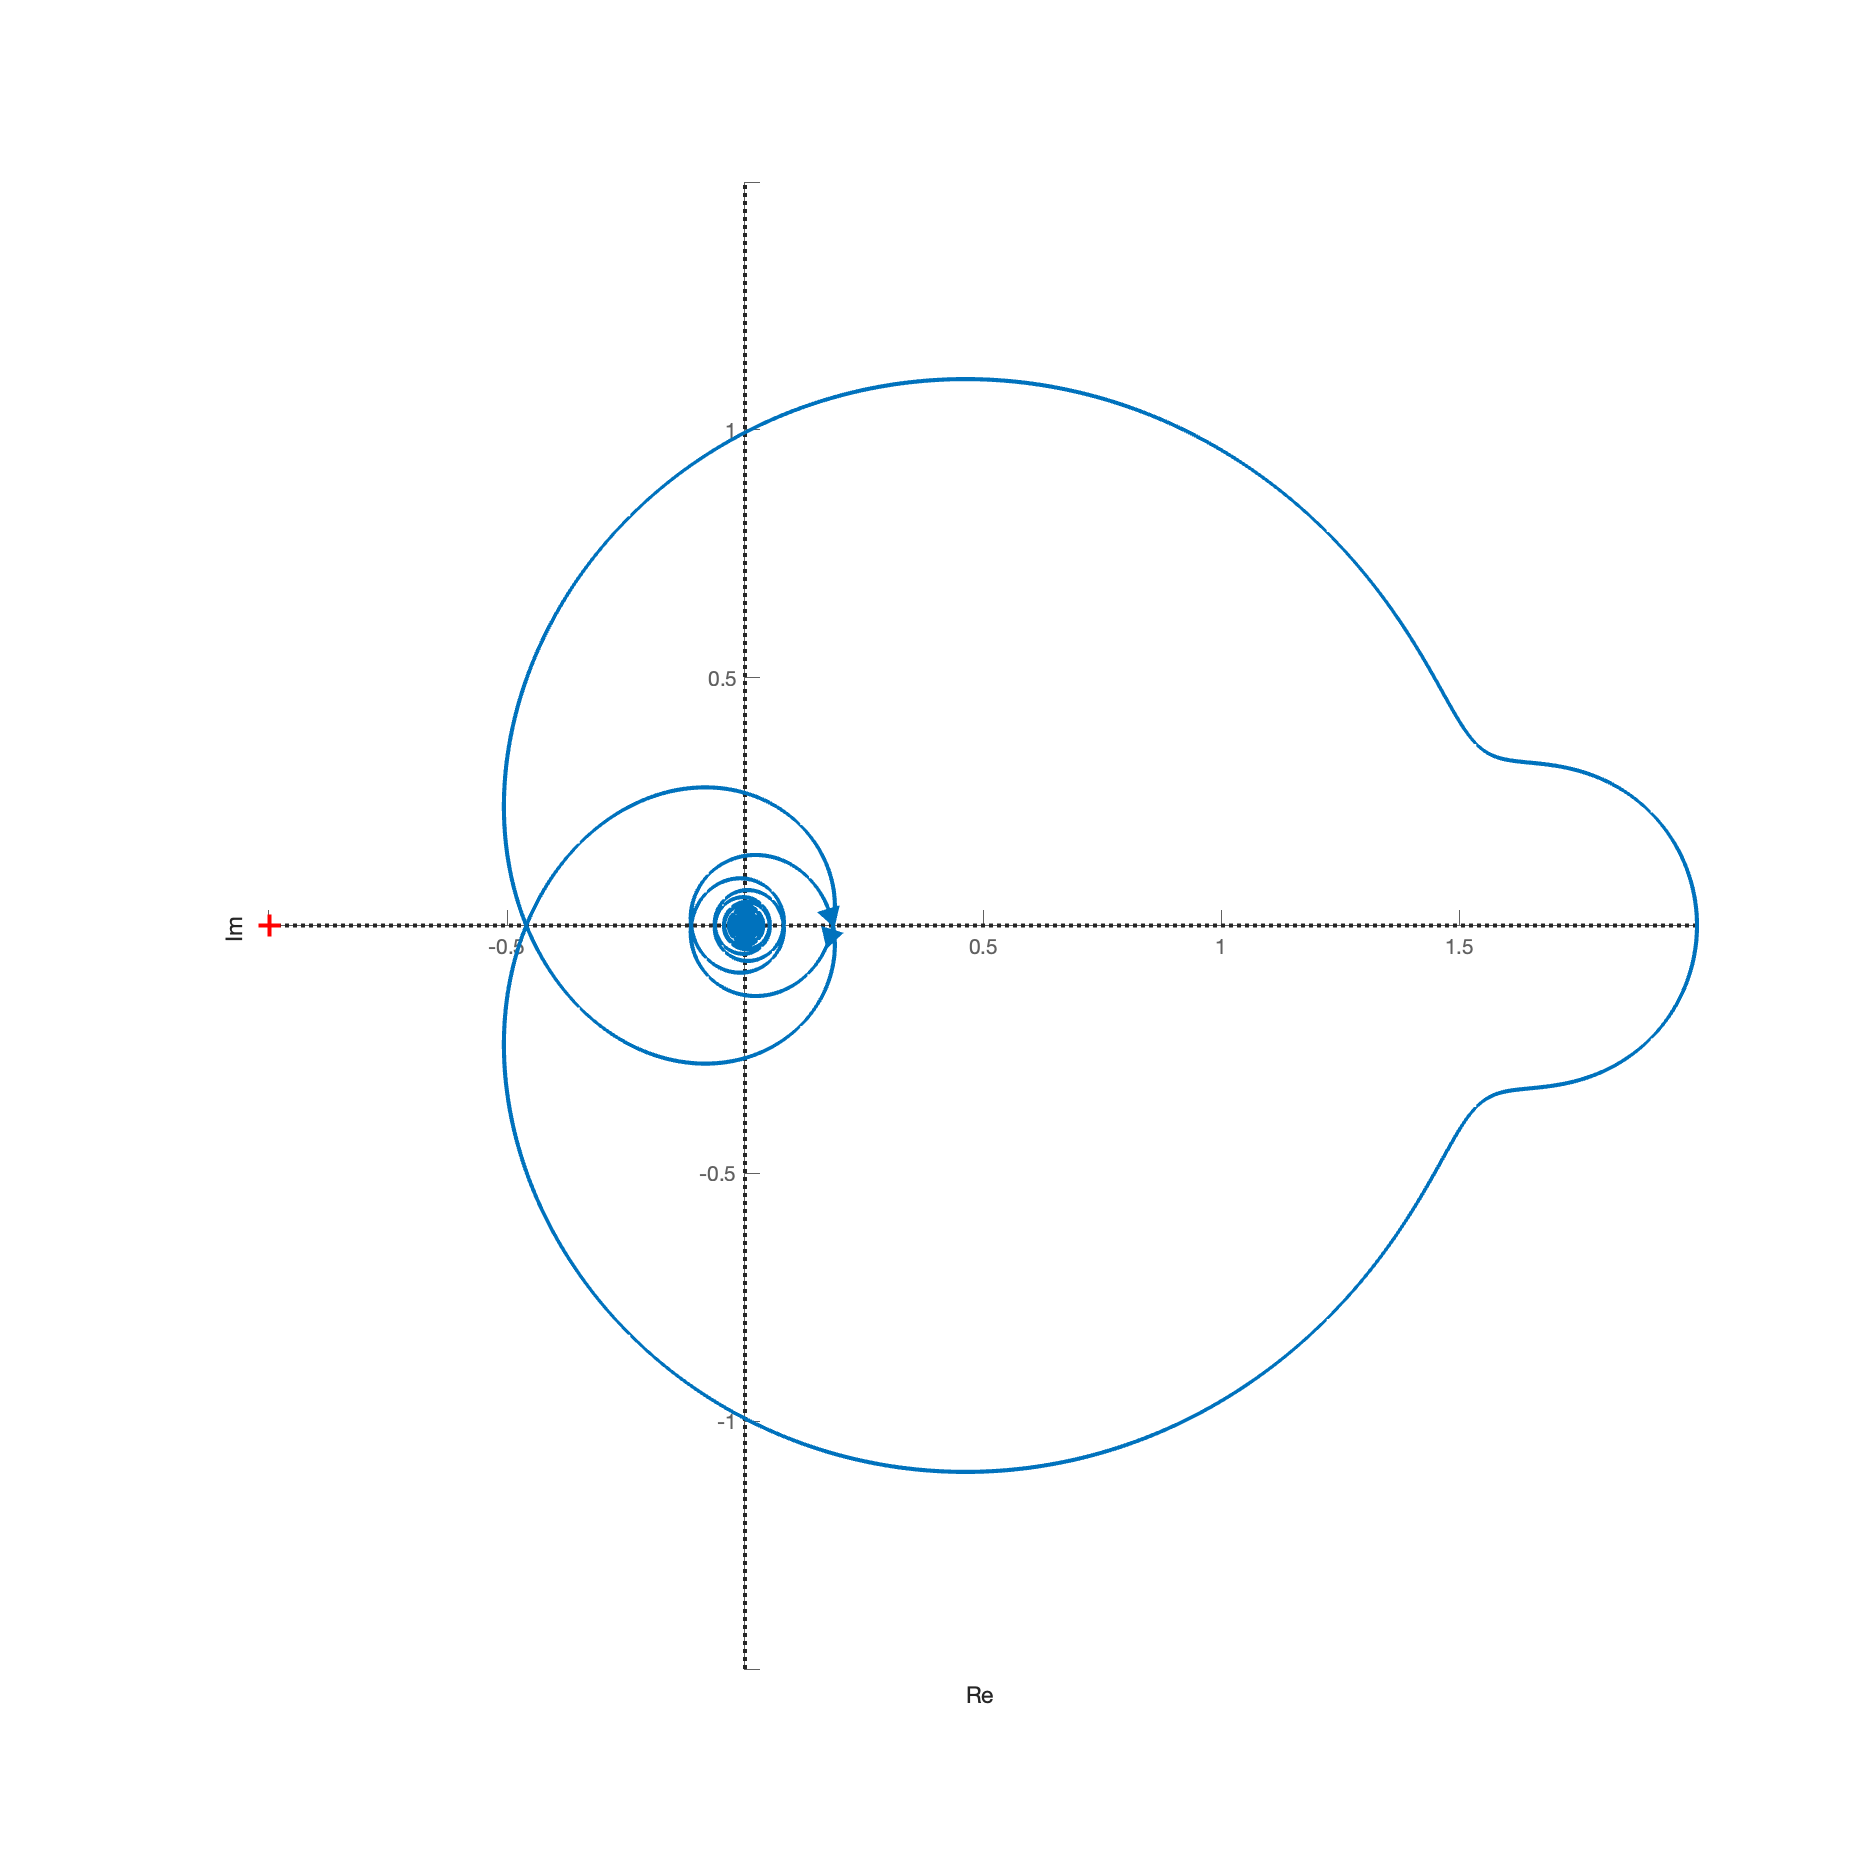
\includegraphics[width=\textwidth]{media/plots/task6_nyquist_open_2.png}
         \caption{$\tau = 0.1$}
    \end{subfigure}
    \begin{subfigure}[b]{0.5\textwidth}
         \centering
         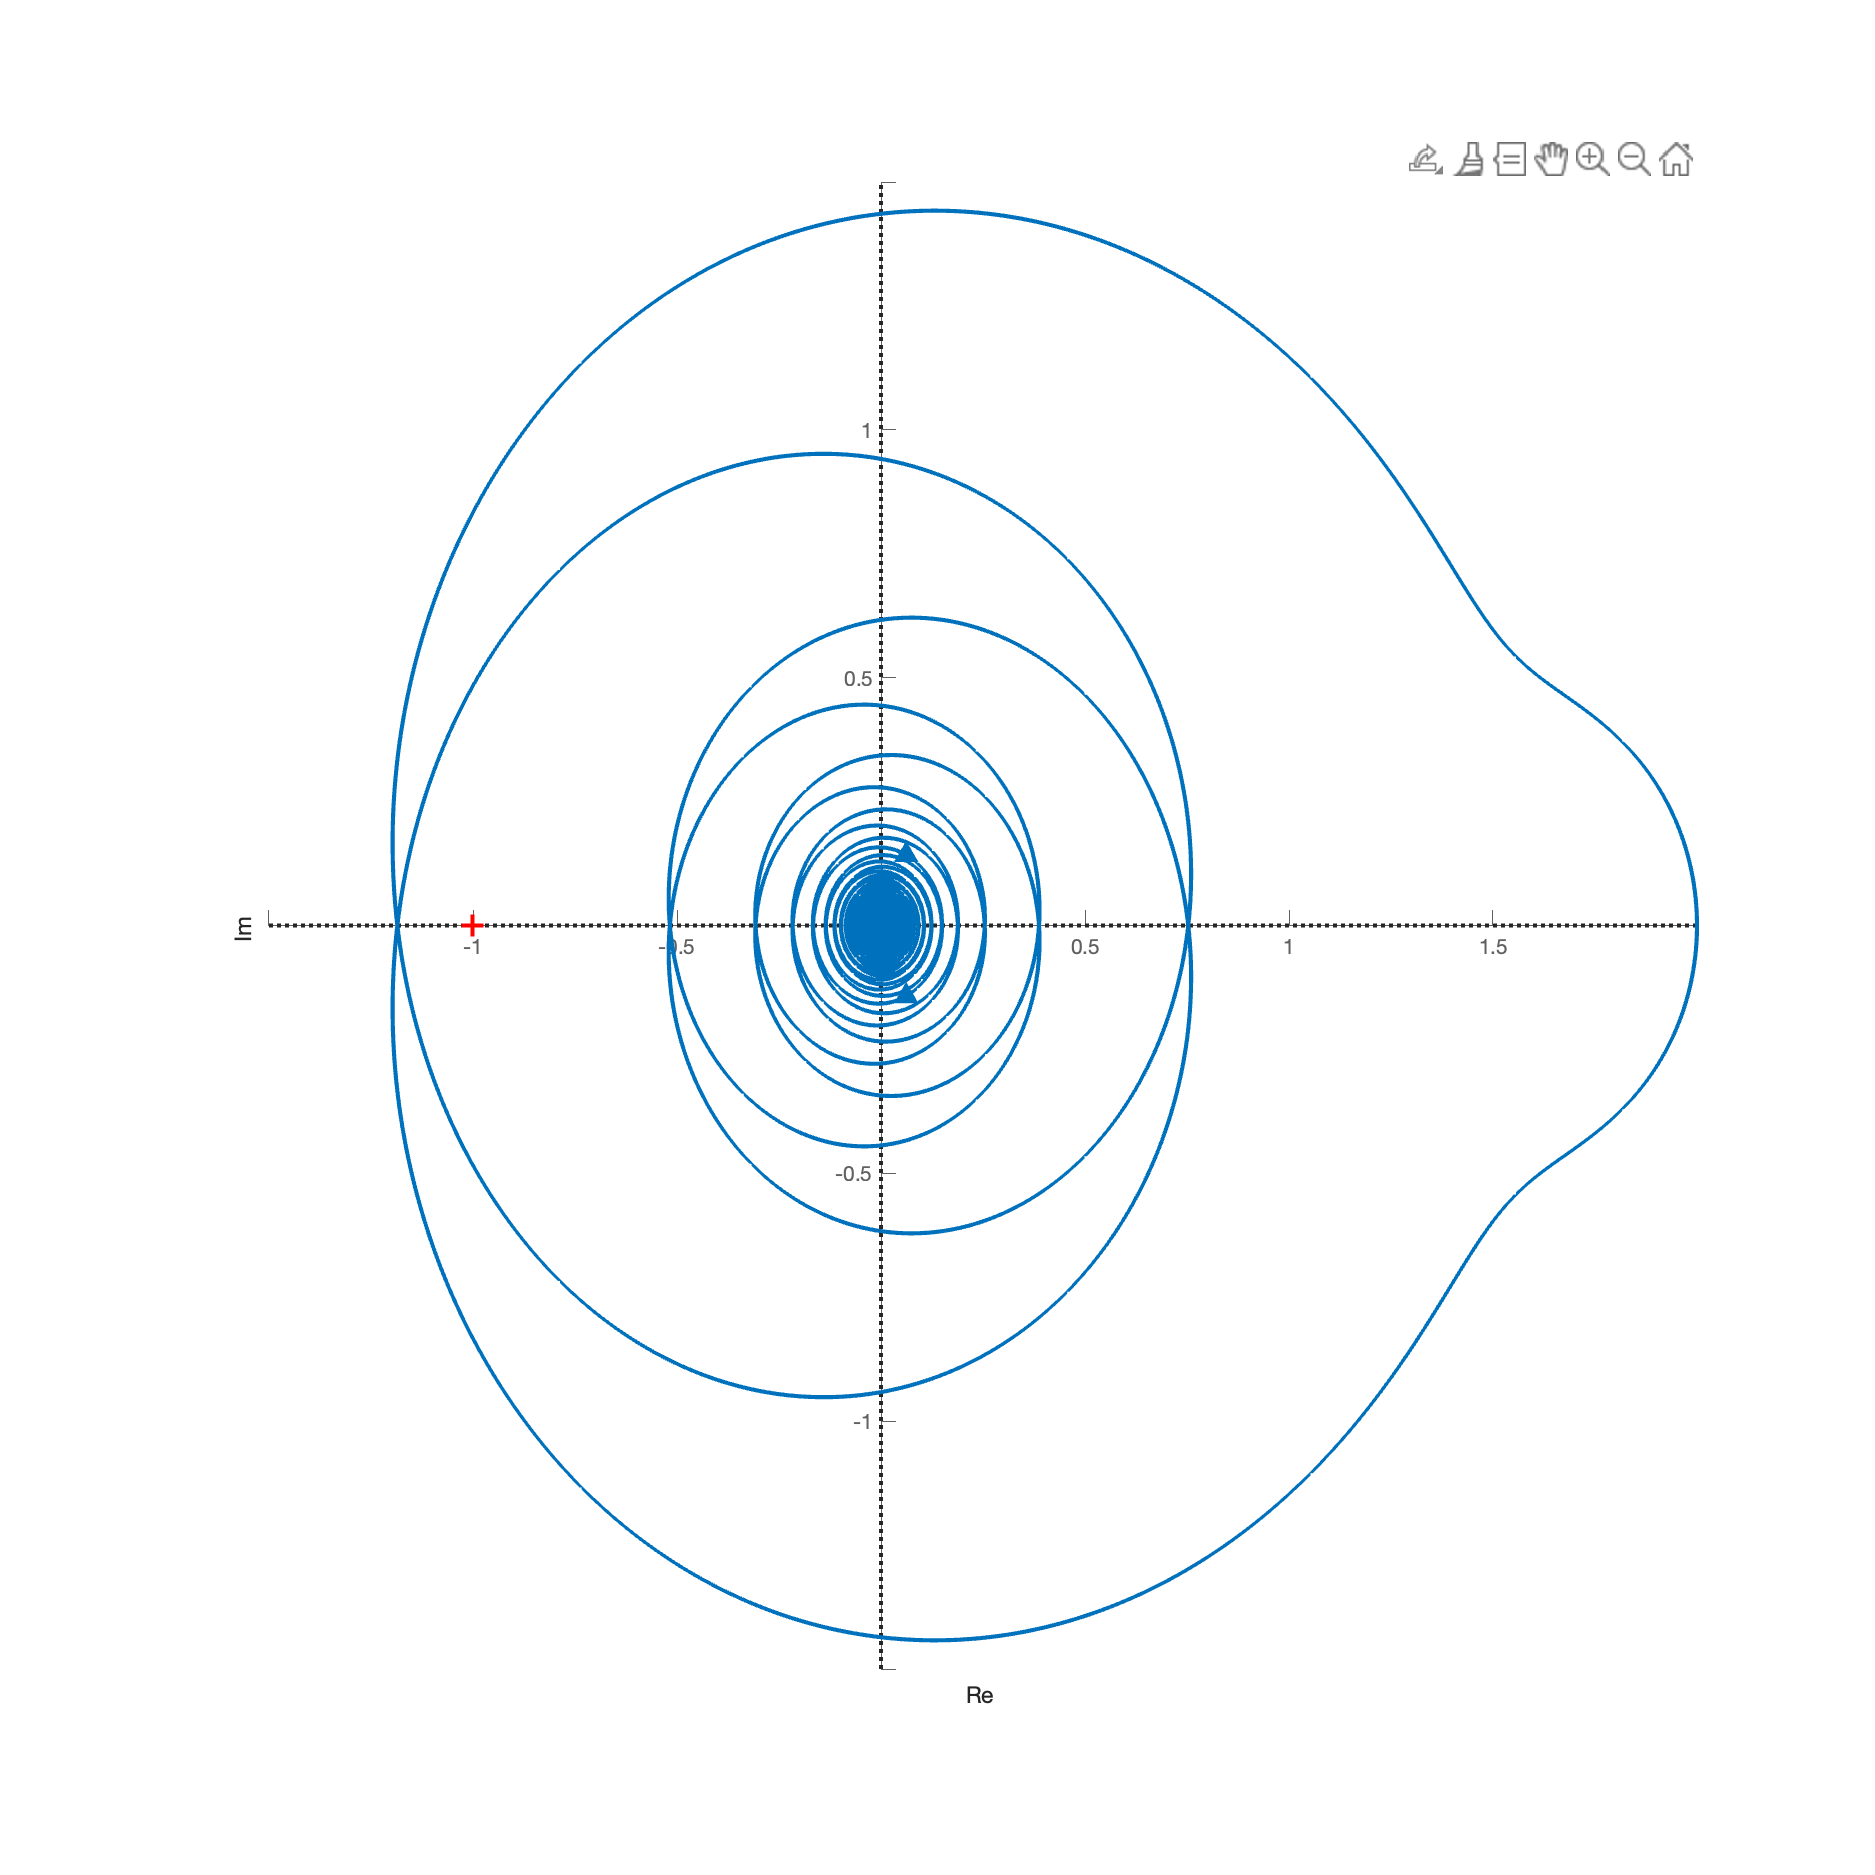
\includegraphics[width=\textwidth]{media/plots/task6_nyquist_open_3.png}
         \caption{$\tau = 0.5$}
    \end{subfigure}
    \begin{subfigure}[b]{0.5\textwidth}
         \centering
         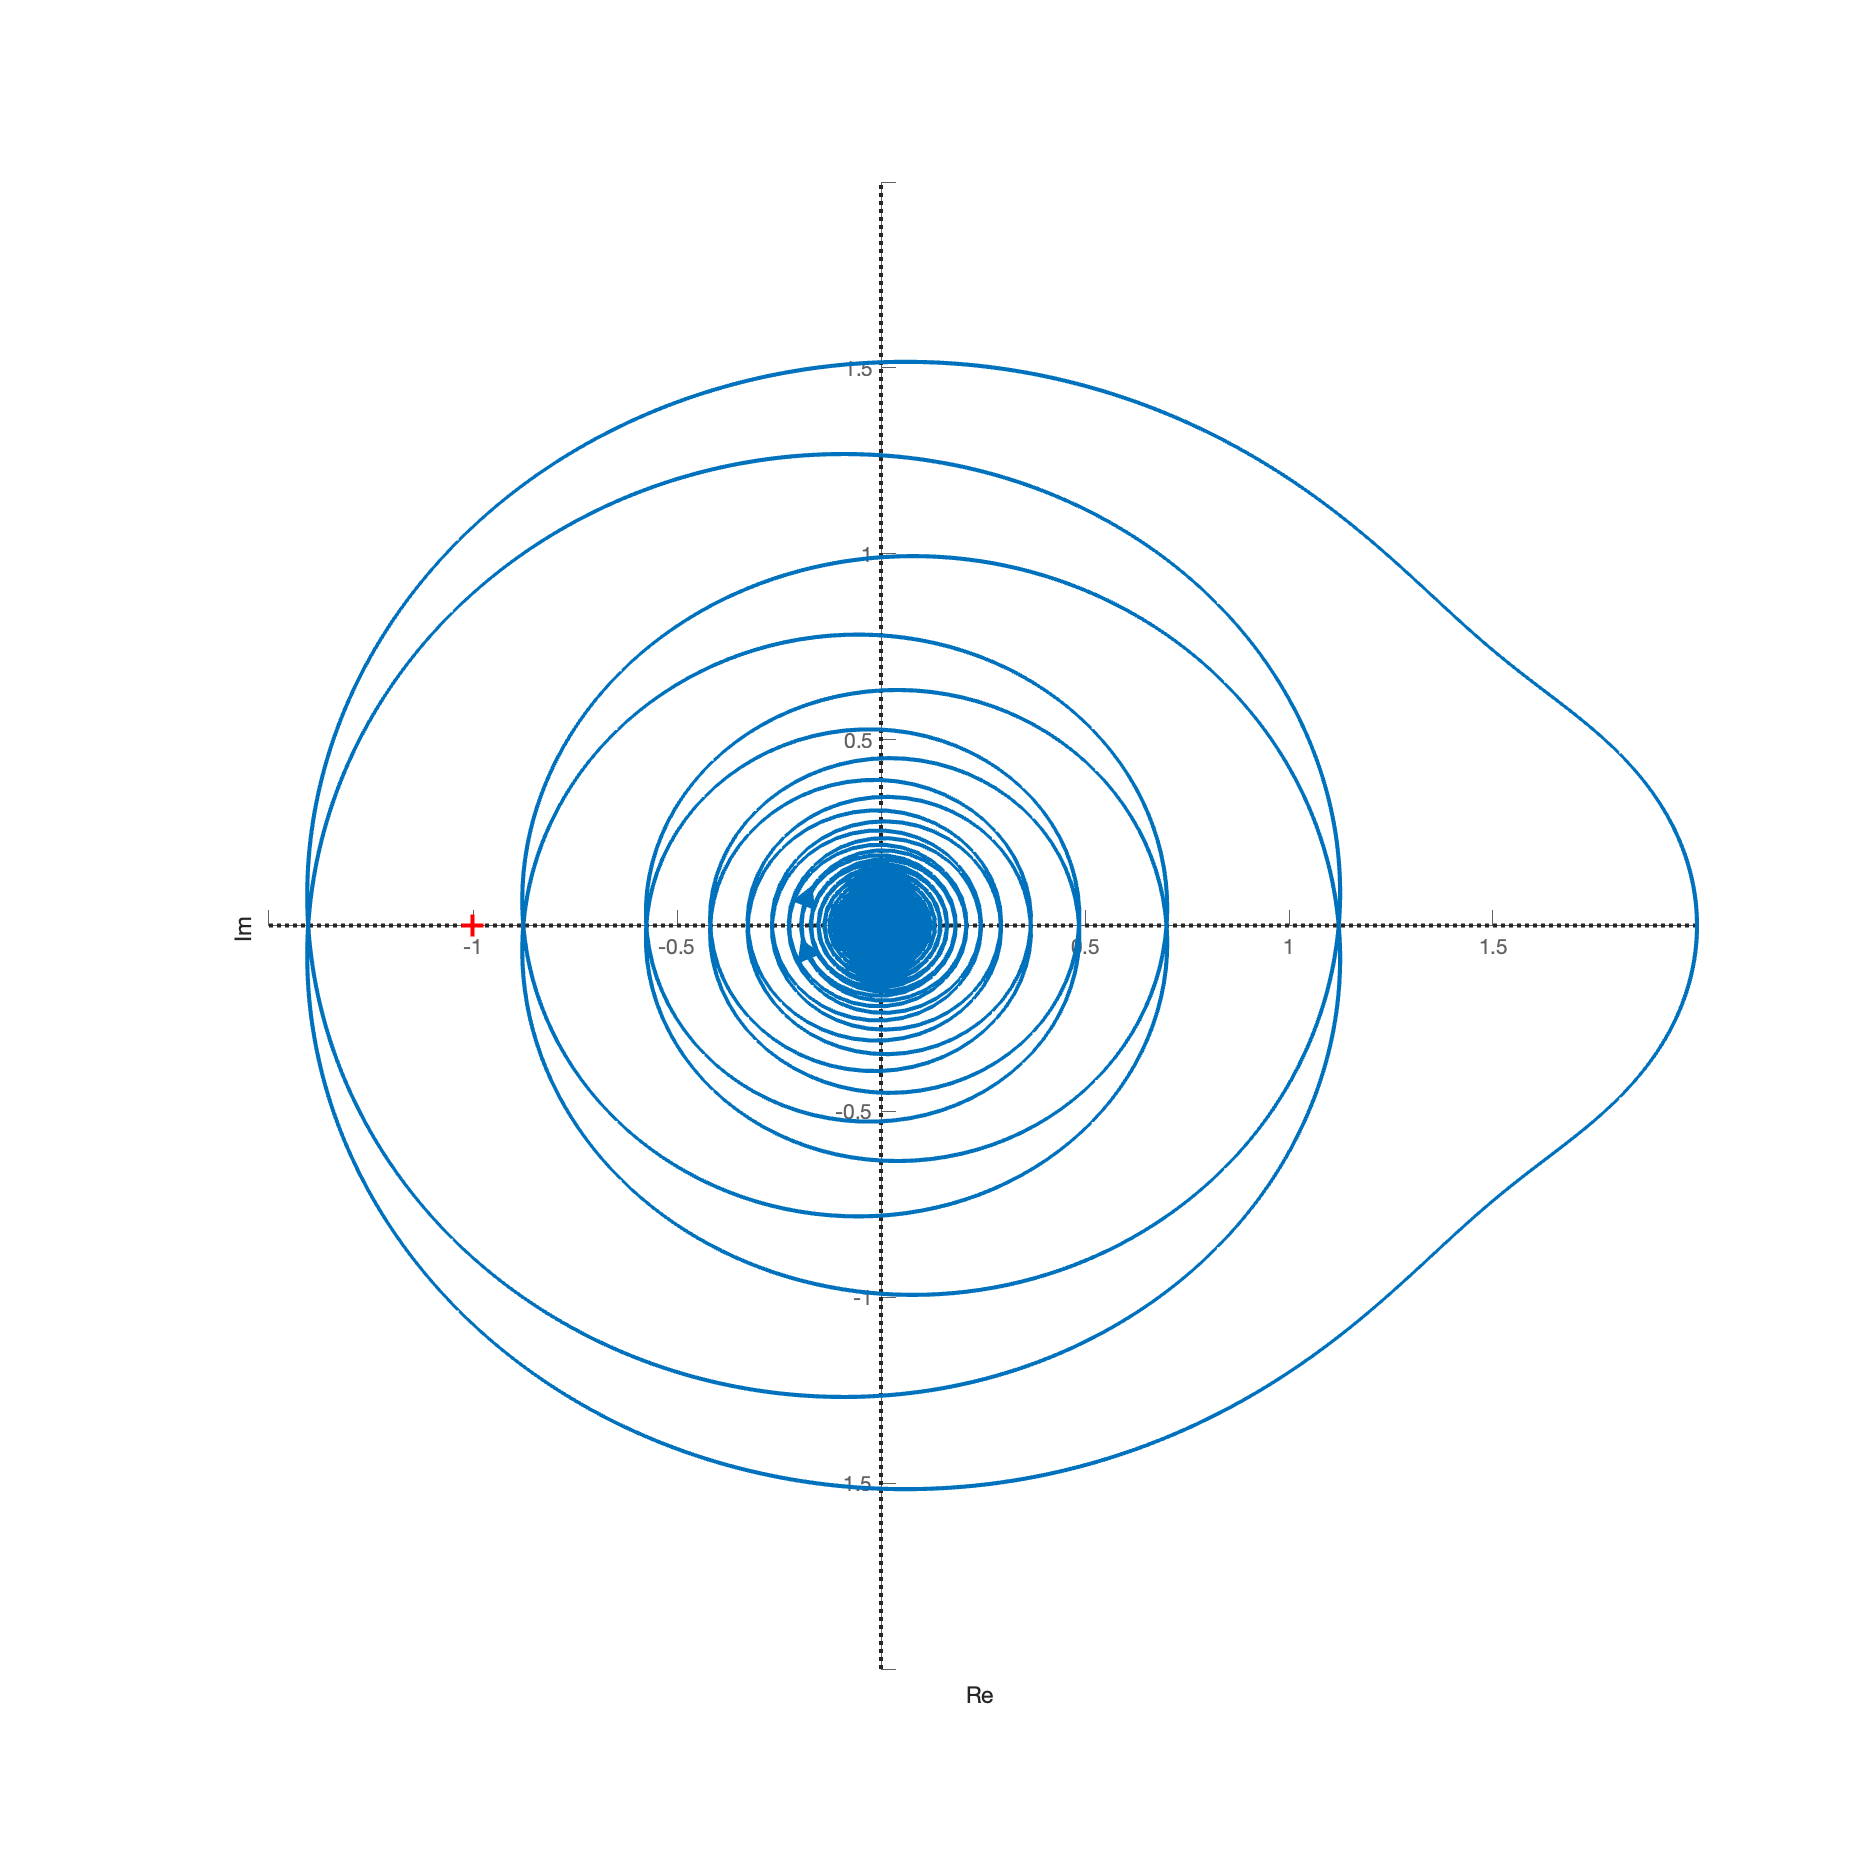
\includegraphics[width=\textwidth]{media/plots/task6_nyquist_open_4.png}
         \caption{$\tau = 1$}
    \end{subfigure}
    \caption{Годограф Найквиста для системы 1}
    \label{fig:task6_niquist}
\end{figure}
Видно, что при увеличении запаздывания $\tau$ годограф закручивается вокруг начала координат сильнее. 
Начиная с какого-то значения $\tau$ годограф начинает оборачиваться вокруг точки $(-1, 0)$ по часовой стрелке,
делая тем самым систему неустойчивой.
Число оборотов растет с увеличением $\tau$. 

Найдем передаточную функцию замкнутой системы: 
\begin{equation}
    W_{1c}(s) = \frac{9s + 2}{s^2 + 6s + 1 + (9s + 2)e^{-\tau s}}e^{-\tau s} = \frac{9s + 2}{s^2 + (6 + 9e^{-\tau s})s + 1 + 2e^{-\tau s}} e^{-\tau s}
\end{equation}

Построим ЛАФЧХ разомкнутой системы при $\tau = 0$ (рис. \ref{fig:task6_bode_open_1}).
\begin{figure}[ht!]
    \centering
    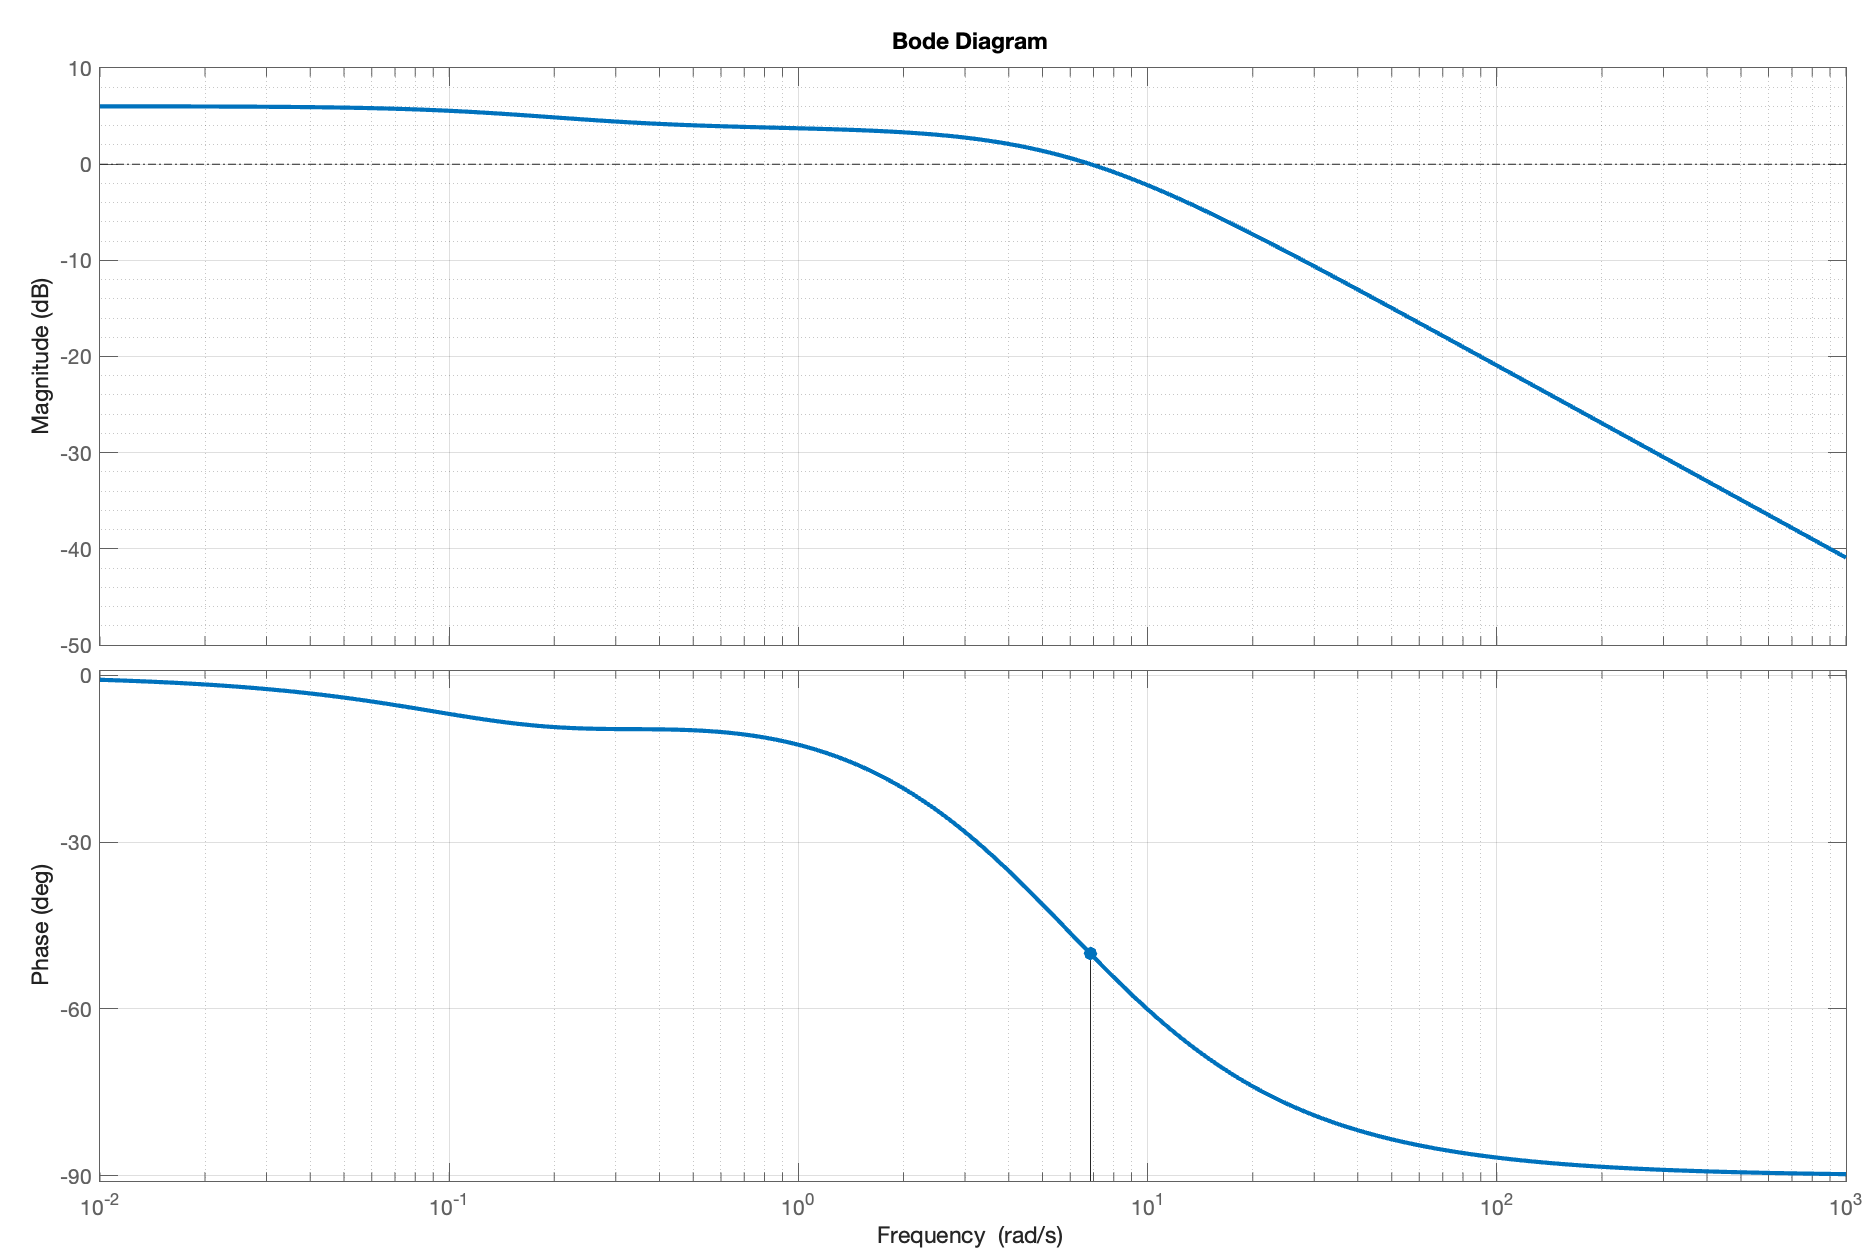
\includegraphics[width=\textwidth]{media/plots/task6_bode_open_1.png}
    \caption{ЛАФЧХ разомкнутой системы 1 при $\tau = 0$}
    \label{fig:task6_bode_open_1}
\end{figure}
АЧХ равно единице при частоте $\omega_A = 6.86$, при этом фаза $\approx-50^\circ$. 
Таким образом, запас устойчивости по фазе будет равен $130^\circ = \frac{13}{18}\pi$. 
Найдем критическое значение $\tau$ при котором система станет неустойчивой: 
\begin{equation}
    \tau_c = \frac{13\pi}{18 \cdot 6.86} \approx 0.33s 
\end{equation}

Графики переходных процессов замкнутой системы для различных значений $\tau$ представлены на рис. \ref{fig:task6_step}.
\begin{figure}[ht!]
    \begin{subfigure}{0.5\textwidth}
        \centering
        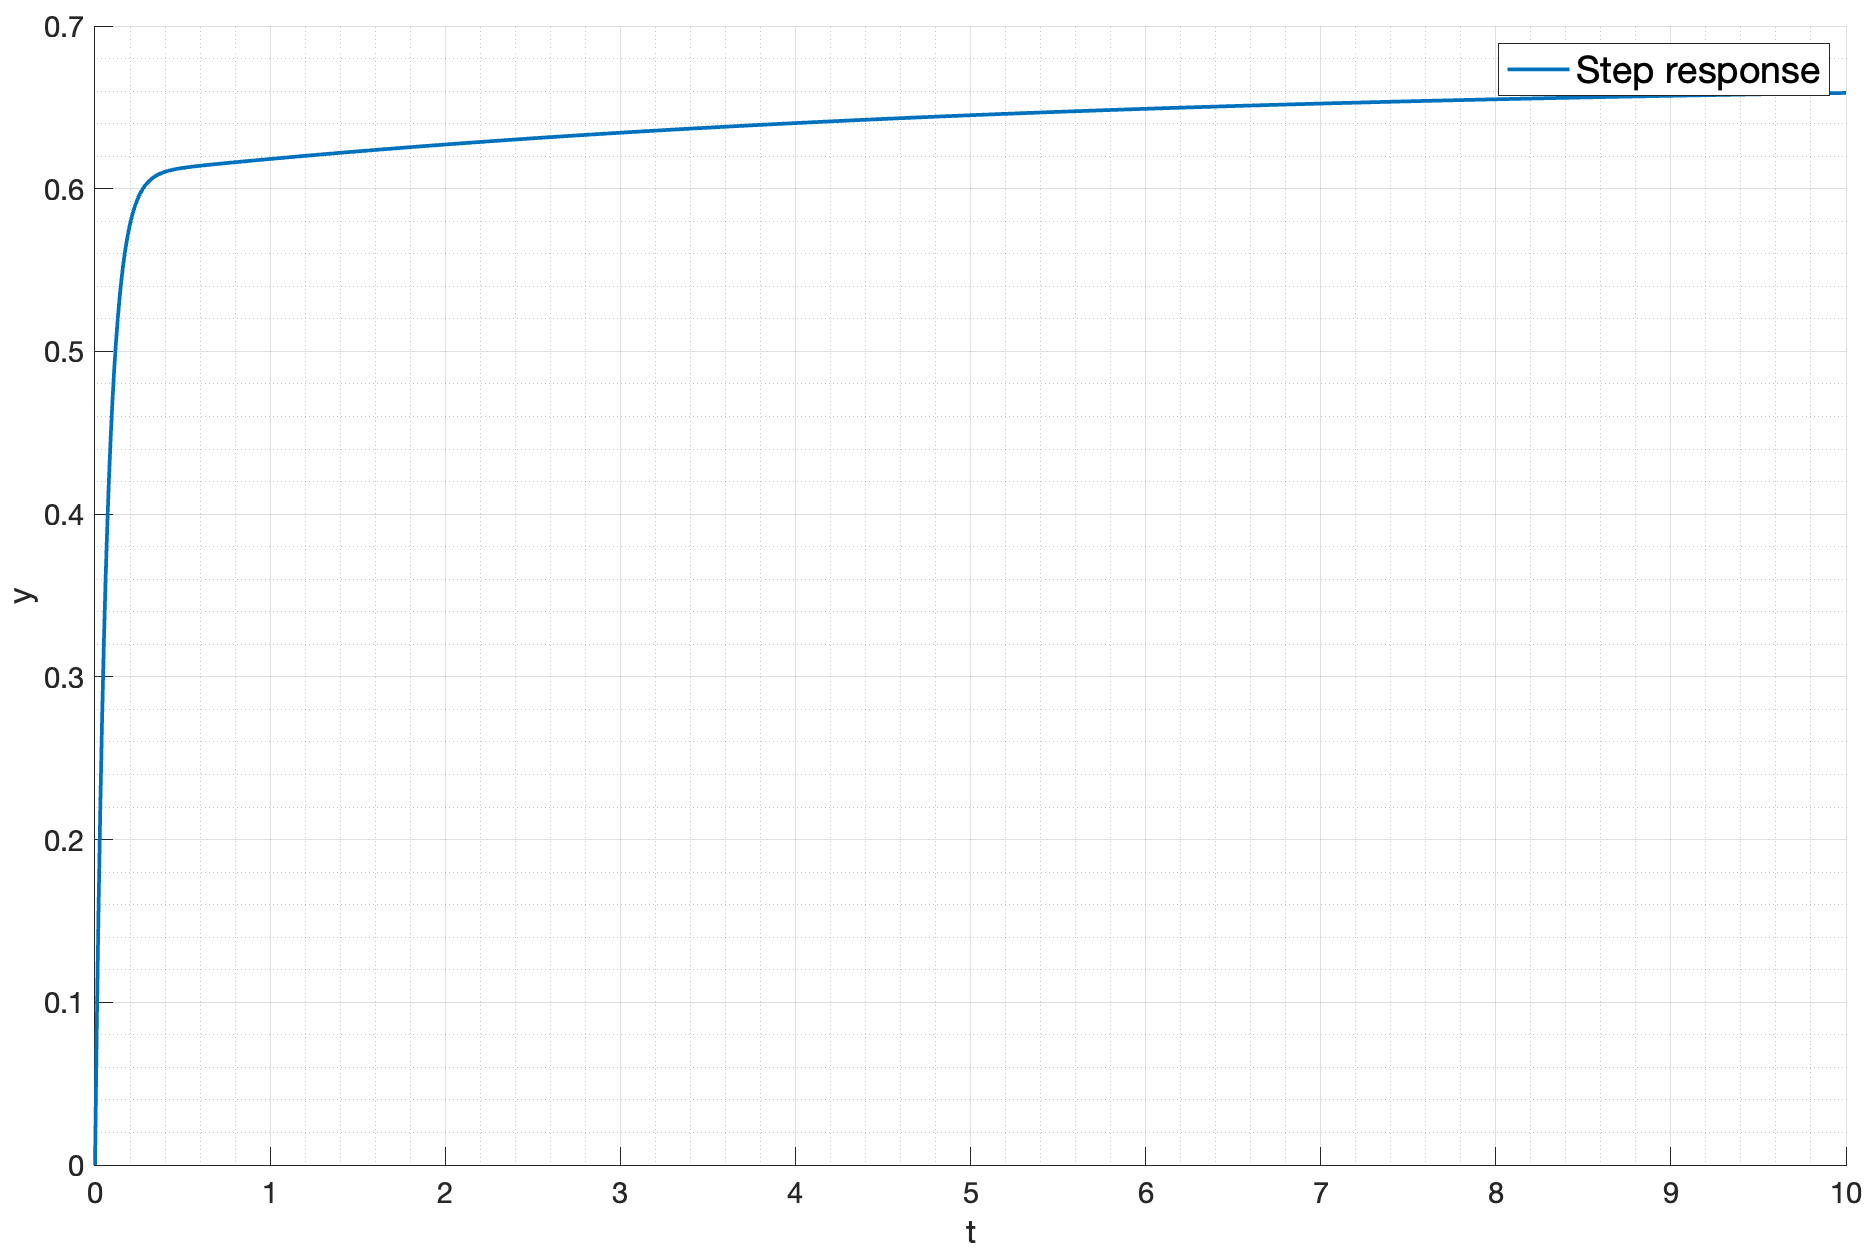
\includegraphics[width=\textwidth]{media/plots/task6_step_response_closed_1.png}
        \caption{$\tau = 0$}
    \end{subfigure}
    \begin{subfigure}{0.5\textwidth}
        \centering
        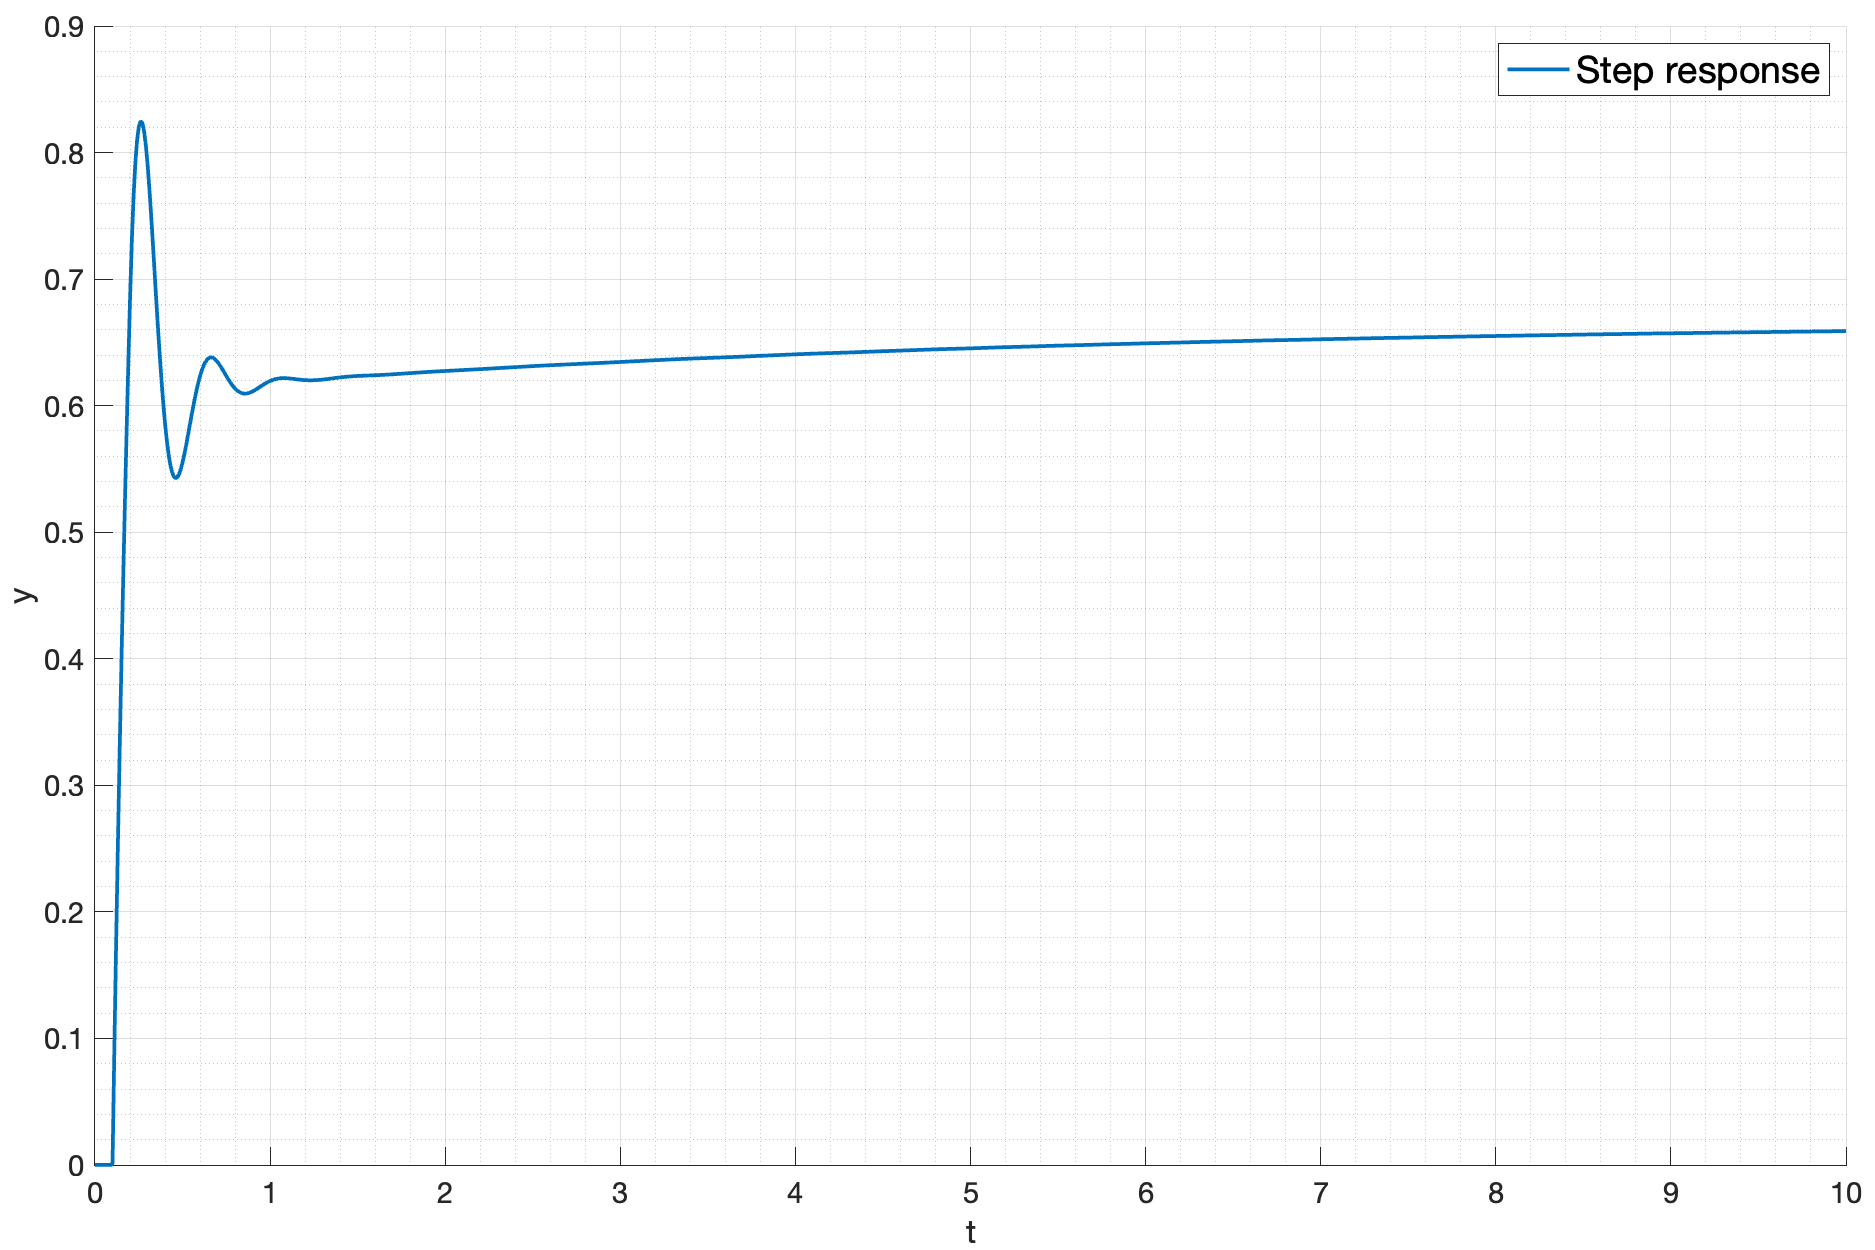
\includegraphics[width=\textwidth]{media/plots/task6_step_response_closed_2.png}
        \caption{$\tau = 0.1$}
    \end{subfigure}
    \begin{subfigure}{0.5\textwidth}
        \centering
        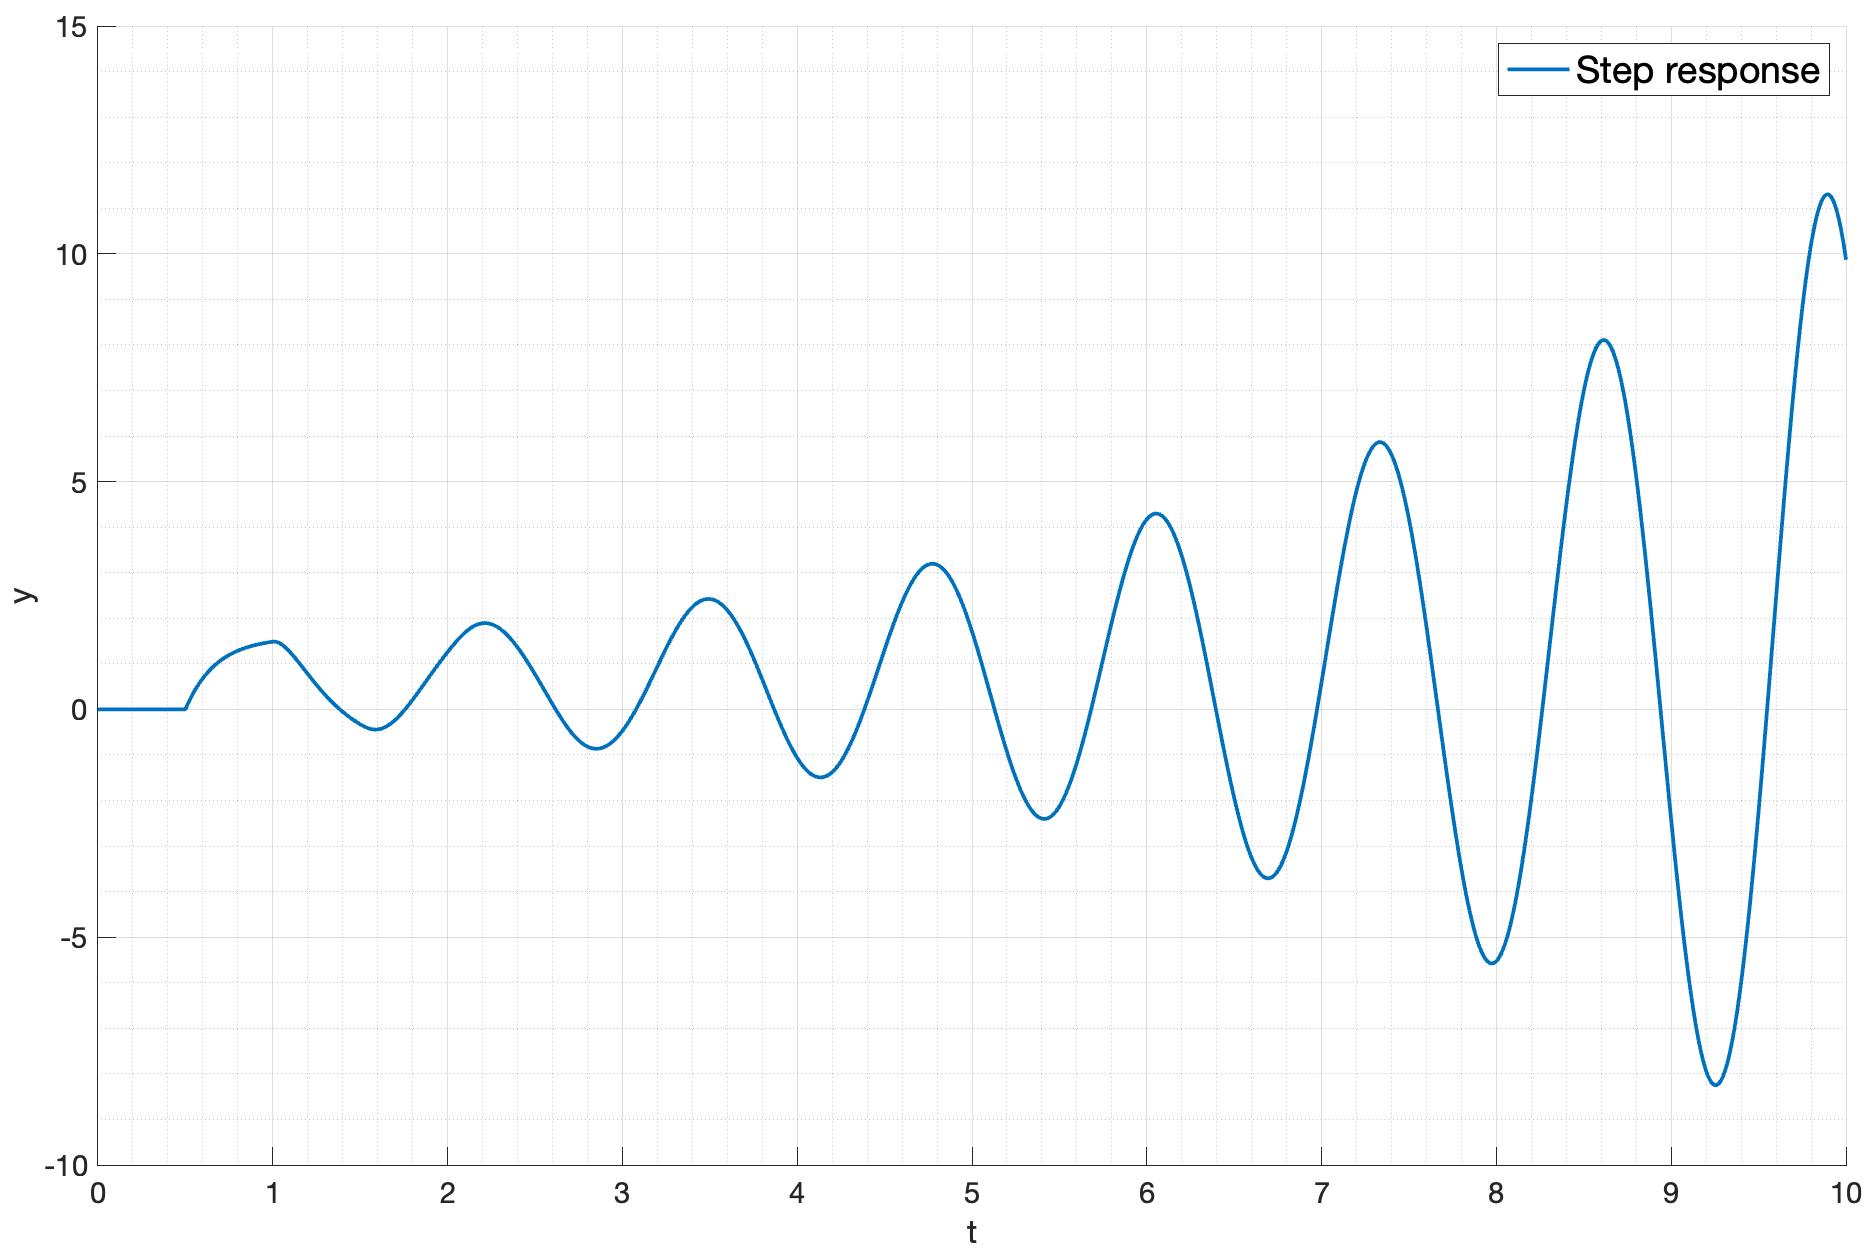
\includegraphics[width=\textwidth]{media/plots/task6_step_response_closed_3.png}
        \caption{$\tau = 0.5$}
    \end{subfigure}
    \begin{subfigure}{0.5\textwidth}
        \centering
        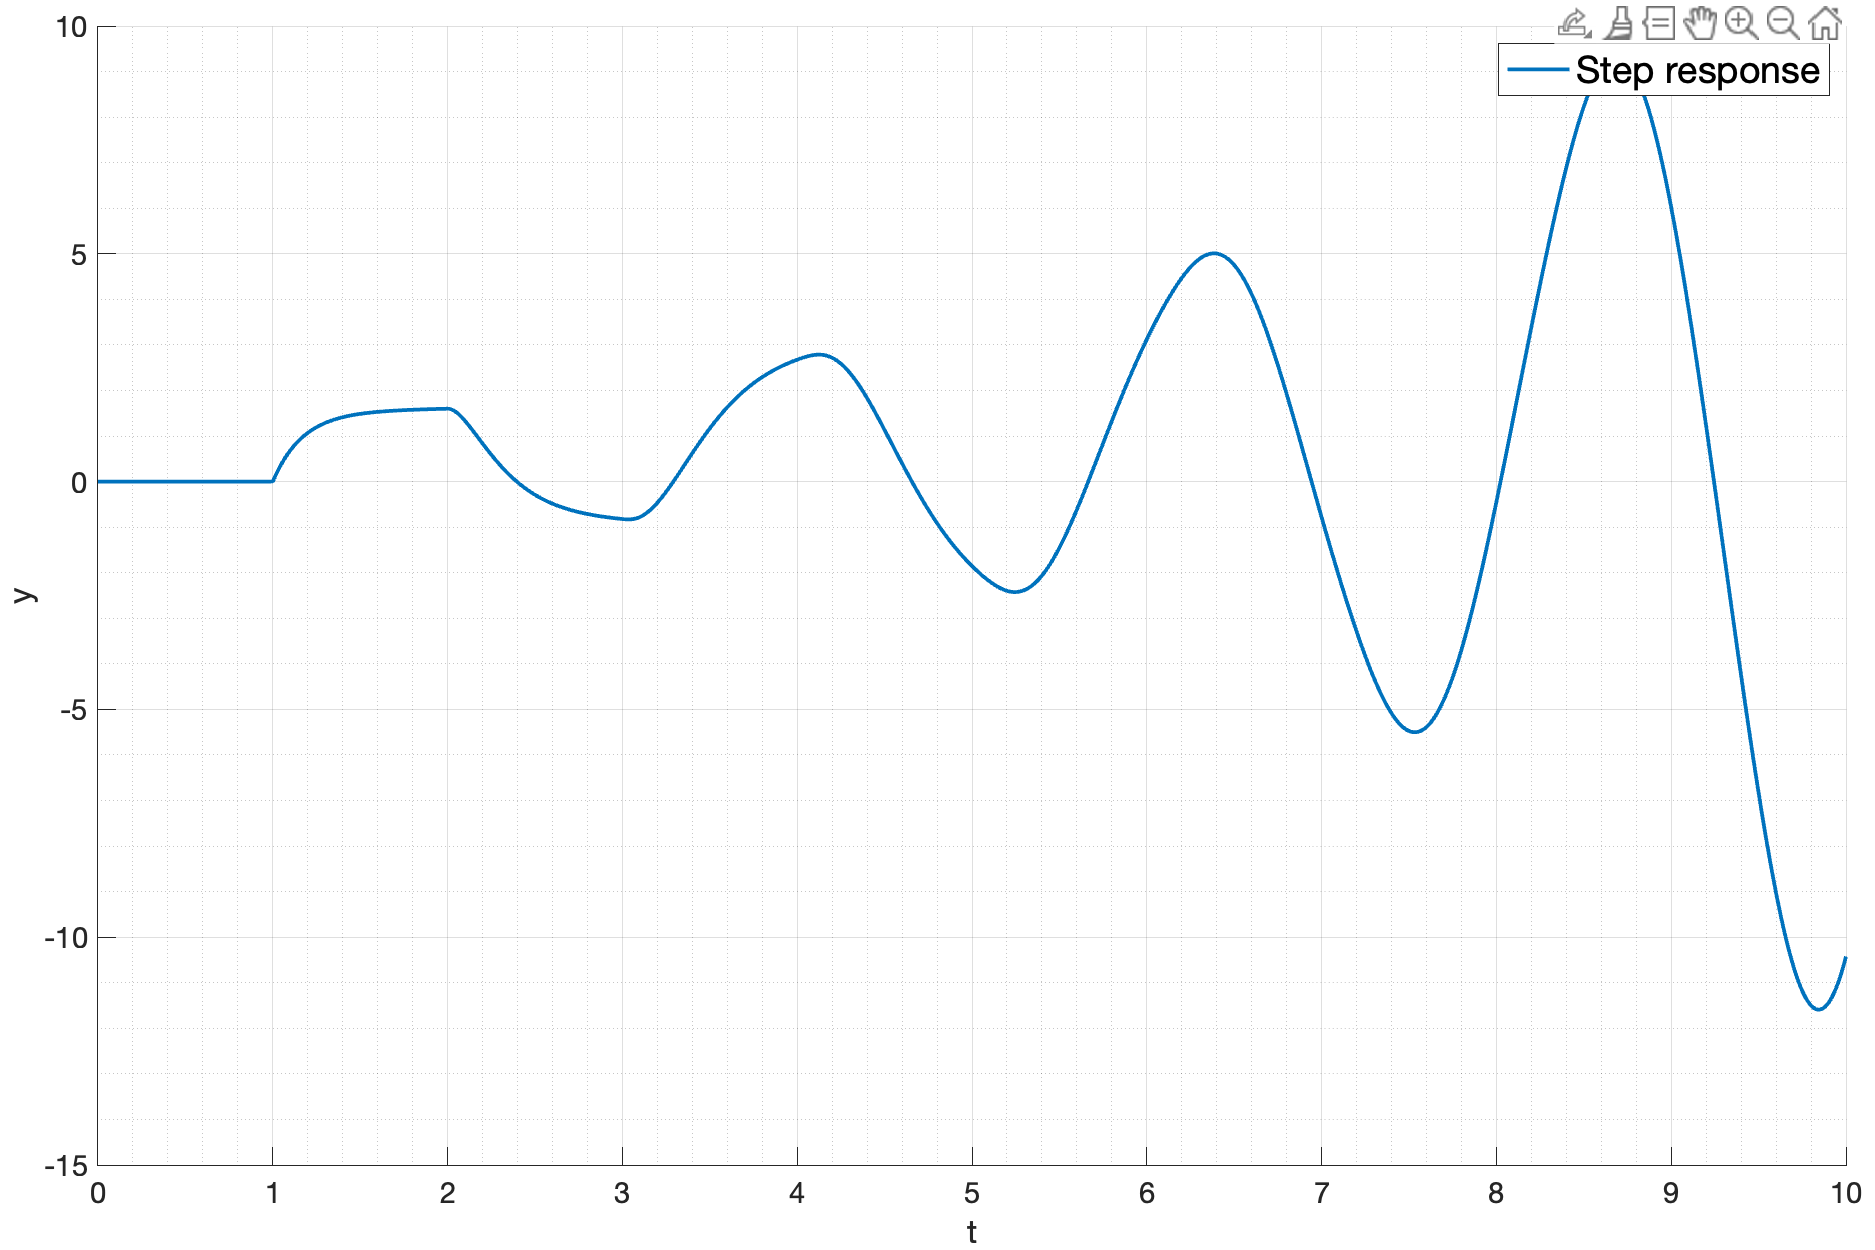
\includegraphics[width=\textwidth]{media/plots/task6_step_response_closed_4.png}
        \caption{$\tau = 1$}
    \end{subfigure}
    \caption{Переходные процессы для системы 1}
    \label{fig:task6_step}
\end{figure}

Видно, что при запаздывании более $0.33s$ система становится неустойчивой. 

\FloatBarrier
\subsection{Система 2}
Рассмотрим систему, заданную передаточной функцией:
\begin{equation}
    W_2(s) = \frac{8s^2 + 4s + 2.4}{10s^2 - 5s + 11} e^{-\tau s}
\end{equation}
Разомкнутая система имеет два неустойчивых полюса:
\begin{equation}
    s_{1,2} = \frac{1}{4} \pm \frac{1}{4}\sqrt{\frac{83}{5}}i
\end{equation}

Построим годограф Найквиста для системы при различных значениях $\tau$ (рис. \ref{fig:task7_niquist}).
\begin{figure}[ht!]
    \begin{subfigure}[b]{0.5\textwidth}
        \centering
        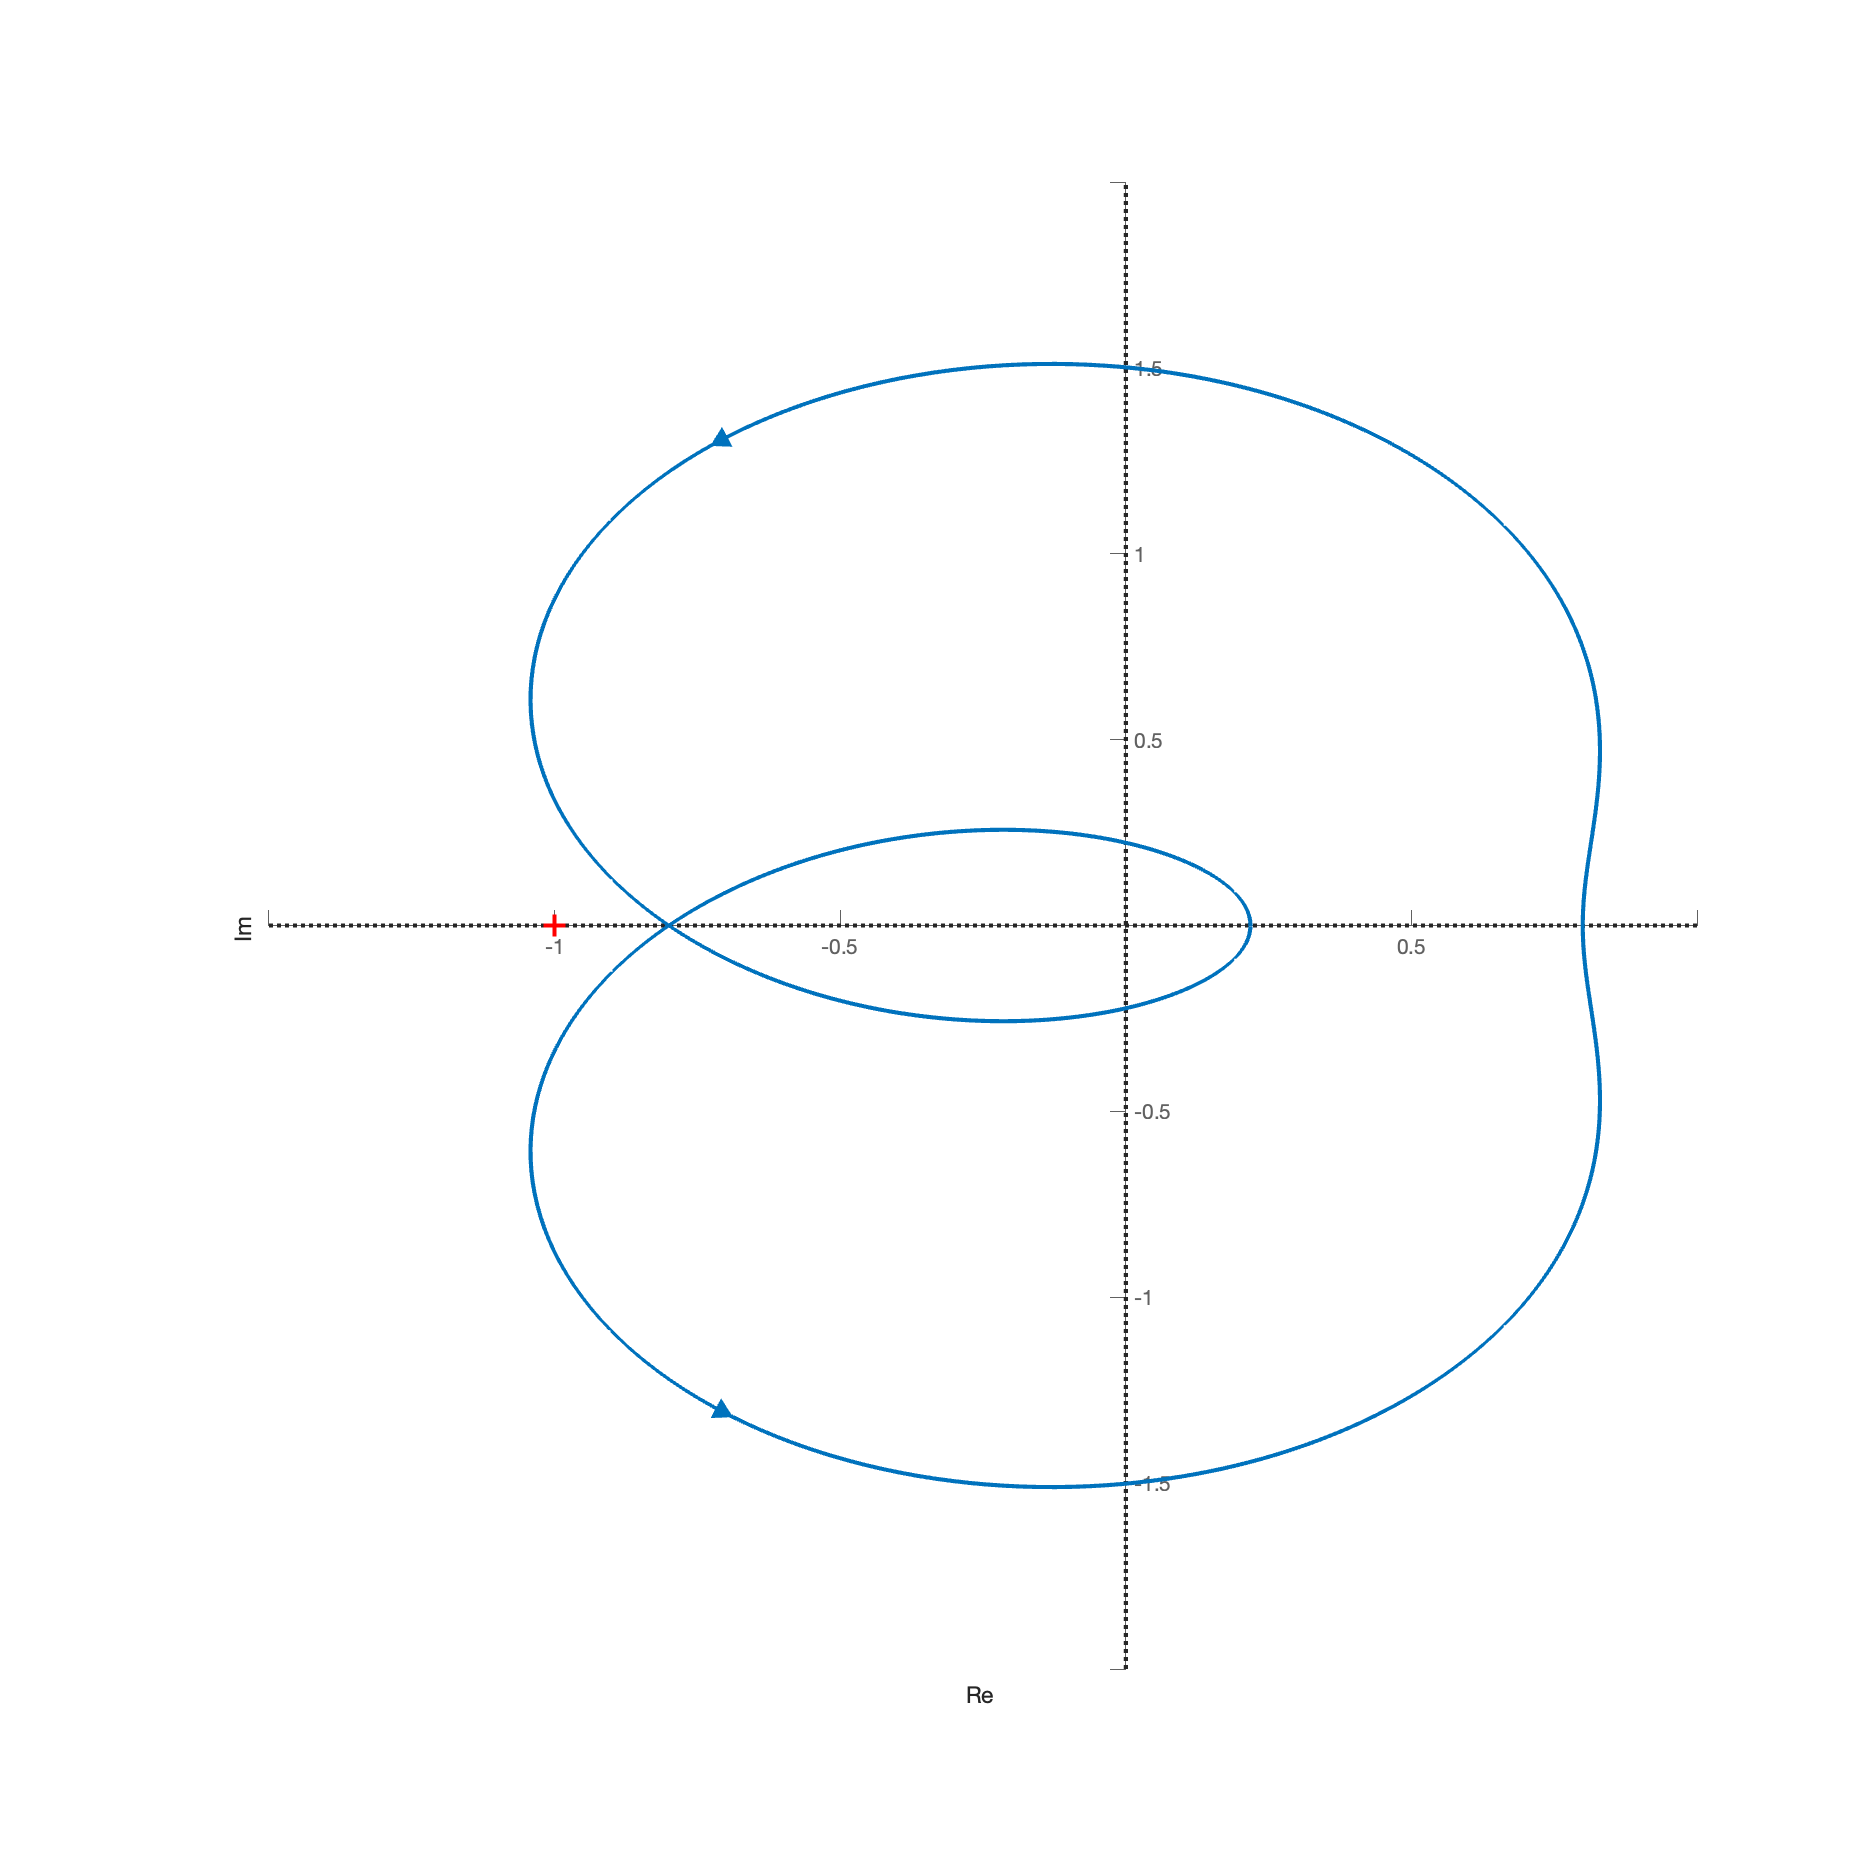
\includegraphics[width=\textwidth]{media/plots/task7_nyquist_open_1.png}
        \caption{$\tau = 0$}
    \end{subfigure}
    \begin{subfigure}[b]{0.5\textwidth}
        \centering
        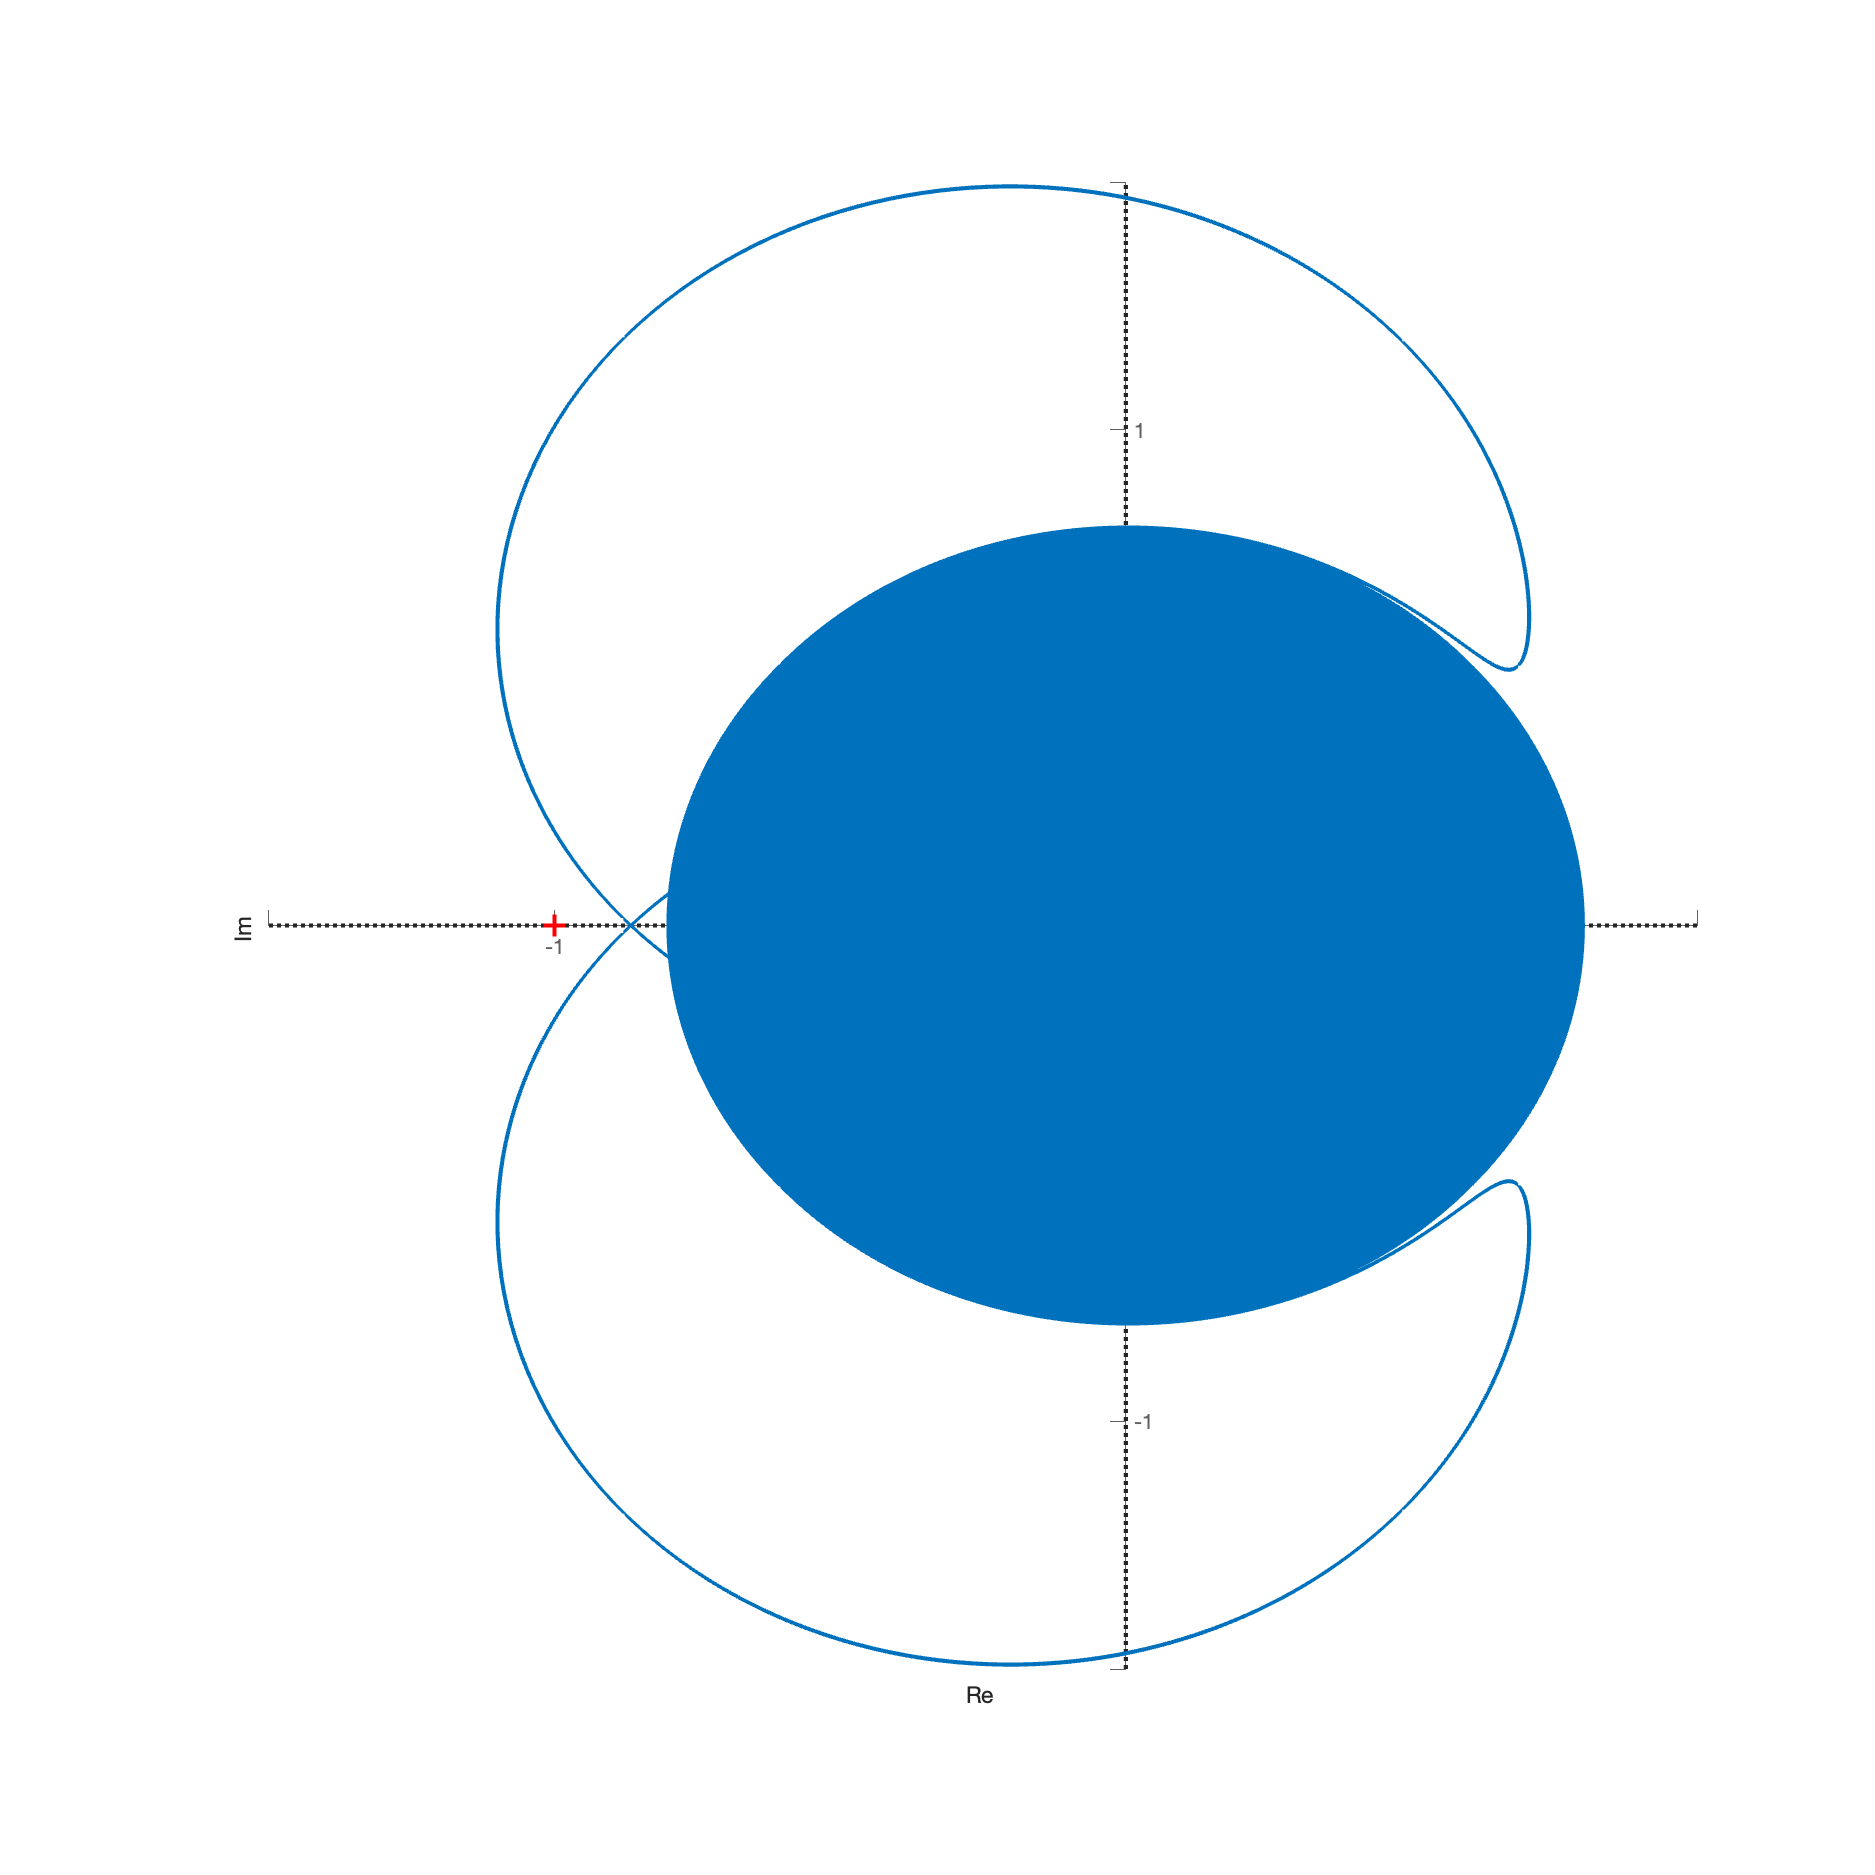
\includegraphics[width=\textwidth]{media/plots/task7_nyquist_open_2.png}
        \caption{$\tau = 0.1$}
    \end{subfigure}
    \begin{subfigure}[b]{0.5\textwidth}
        \centering
        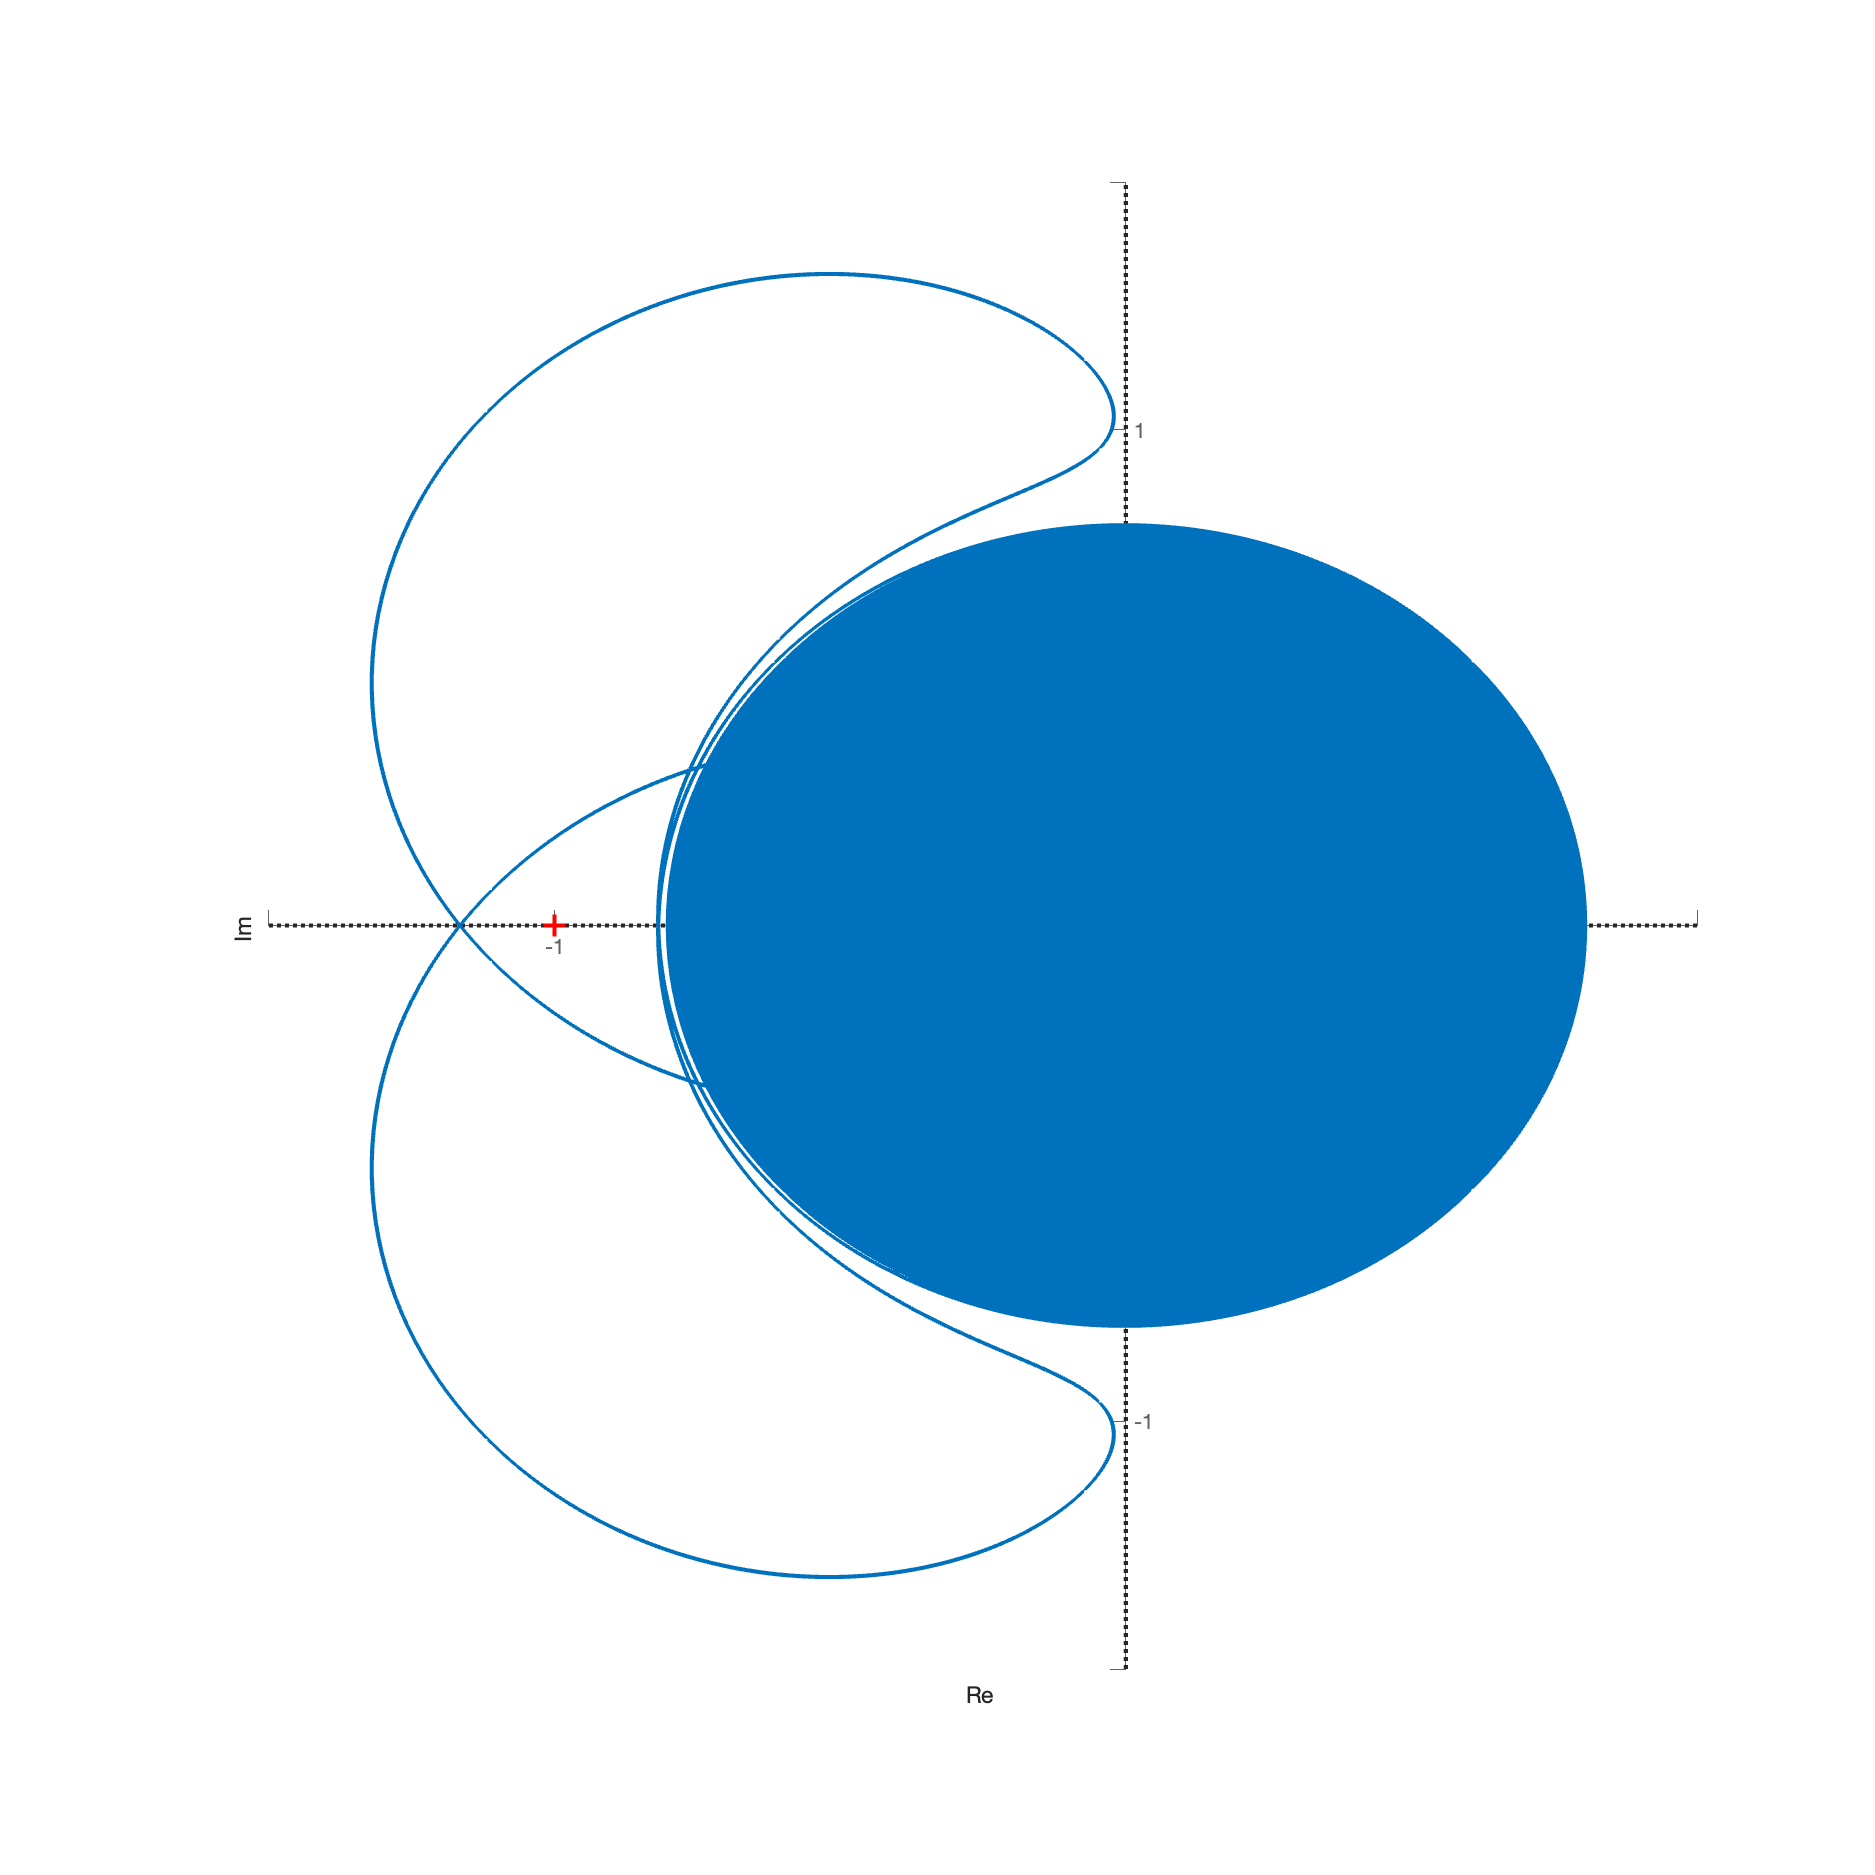
\includegraphics[width=\textwidth]{media/plots/task7_nyquist_open_3.png}
        \caption{$\tau = 0.5$}
    \end{subfigure}
    \begin{subfigure}[b]{0.5\textwidth}
        \centering
        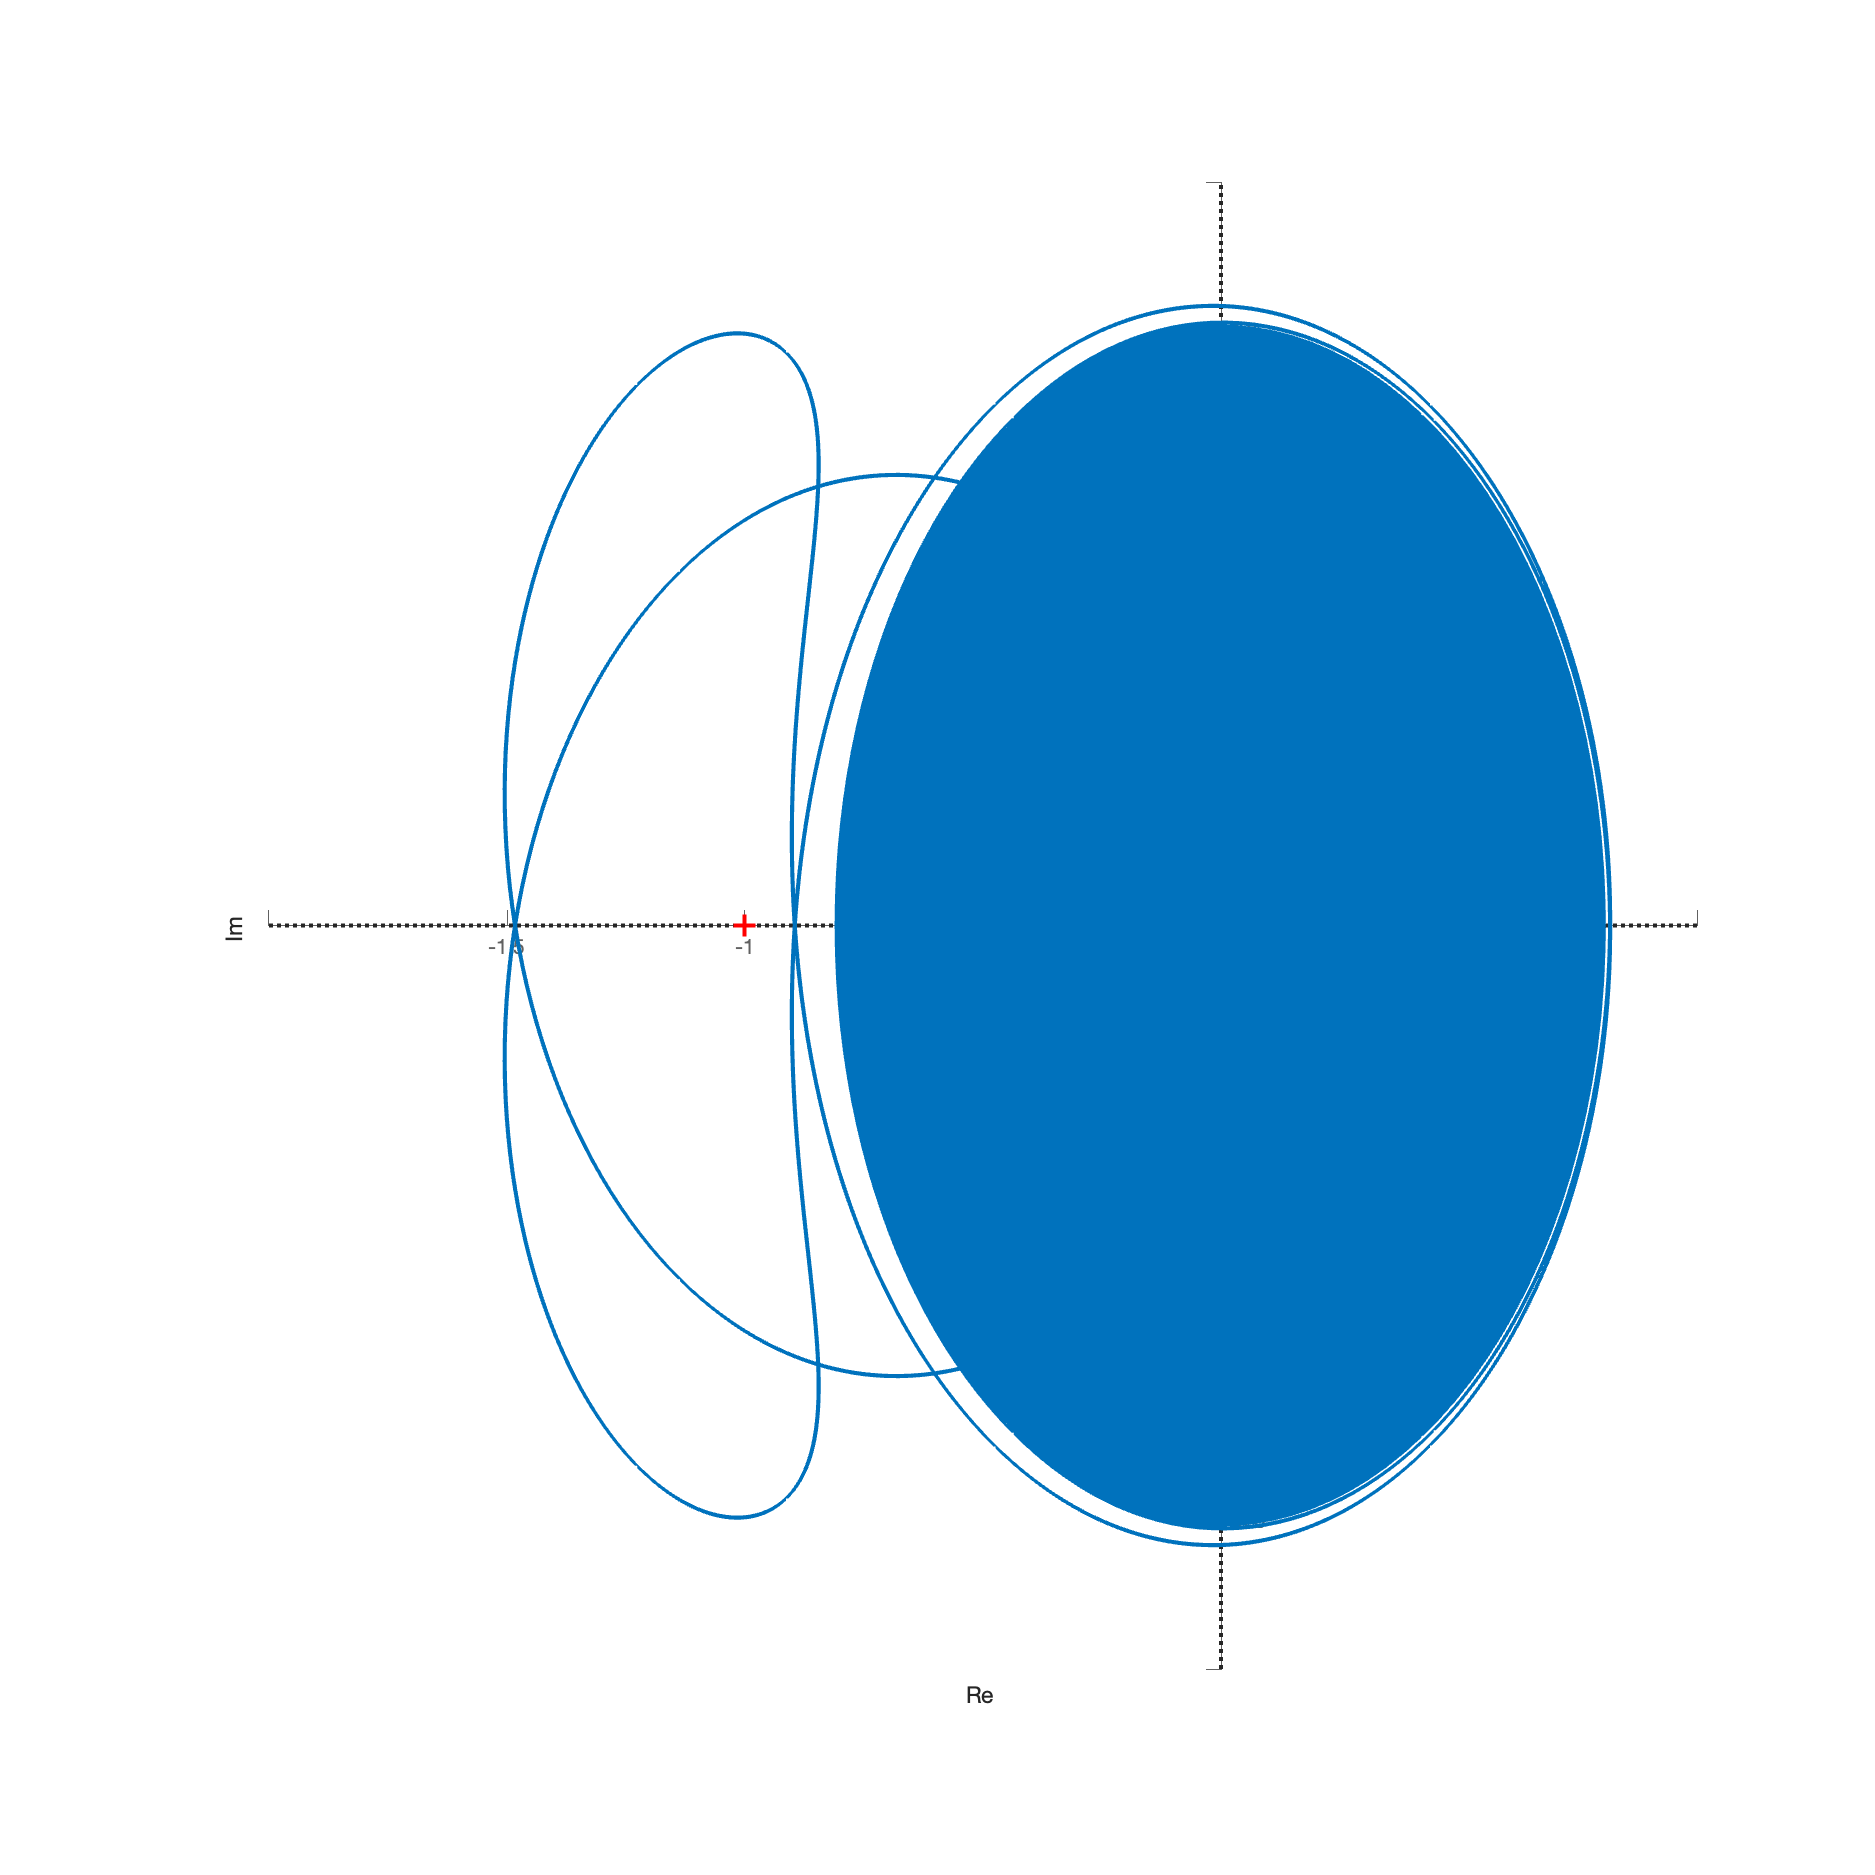
\includegraphics[width=\textwidth]{media/plots/task7_nyquist_open_4.png}
        \caption{$\tau = 1$}
    \end{subfigure}
    \caption{Годограф Найквиста для системы 2}
    \label{fig:task7_niquist}
\end{figure}
Как и в предыдущем случае, при увеличении запаздывания $\tau$ годограф закручивается вокруг начала координат сильнее.

Найдем передаточную функцию замкнутой системы:
\begin{equation}
    W_{2c}(s) = \frac{8s^2 + 4s + 2.4}{(10 + 8 e^{-\tau s})s^2 + (-5 + 4e^{-\tau s})s + 11 + 2.4e^{-\tau s}}e^{-\tau s}
\end{equation}

Построим ЛАФЧХ разомкнутой системы при $\tau = 0$ (рис. \ref{fig:task7_bode_open_1}).
\begin{figure}[ht!]
    \centering
    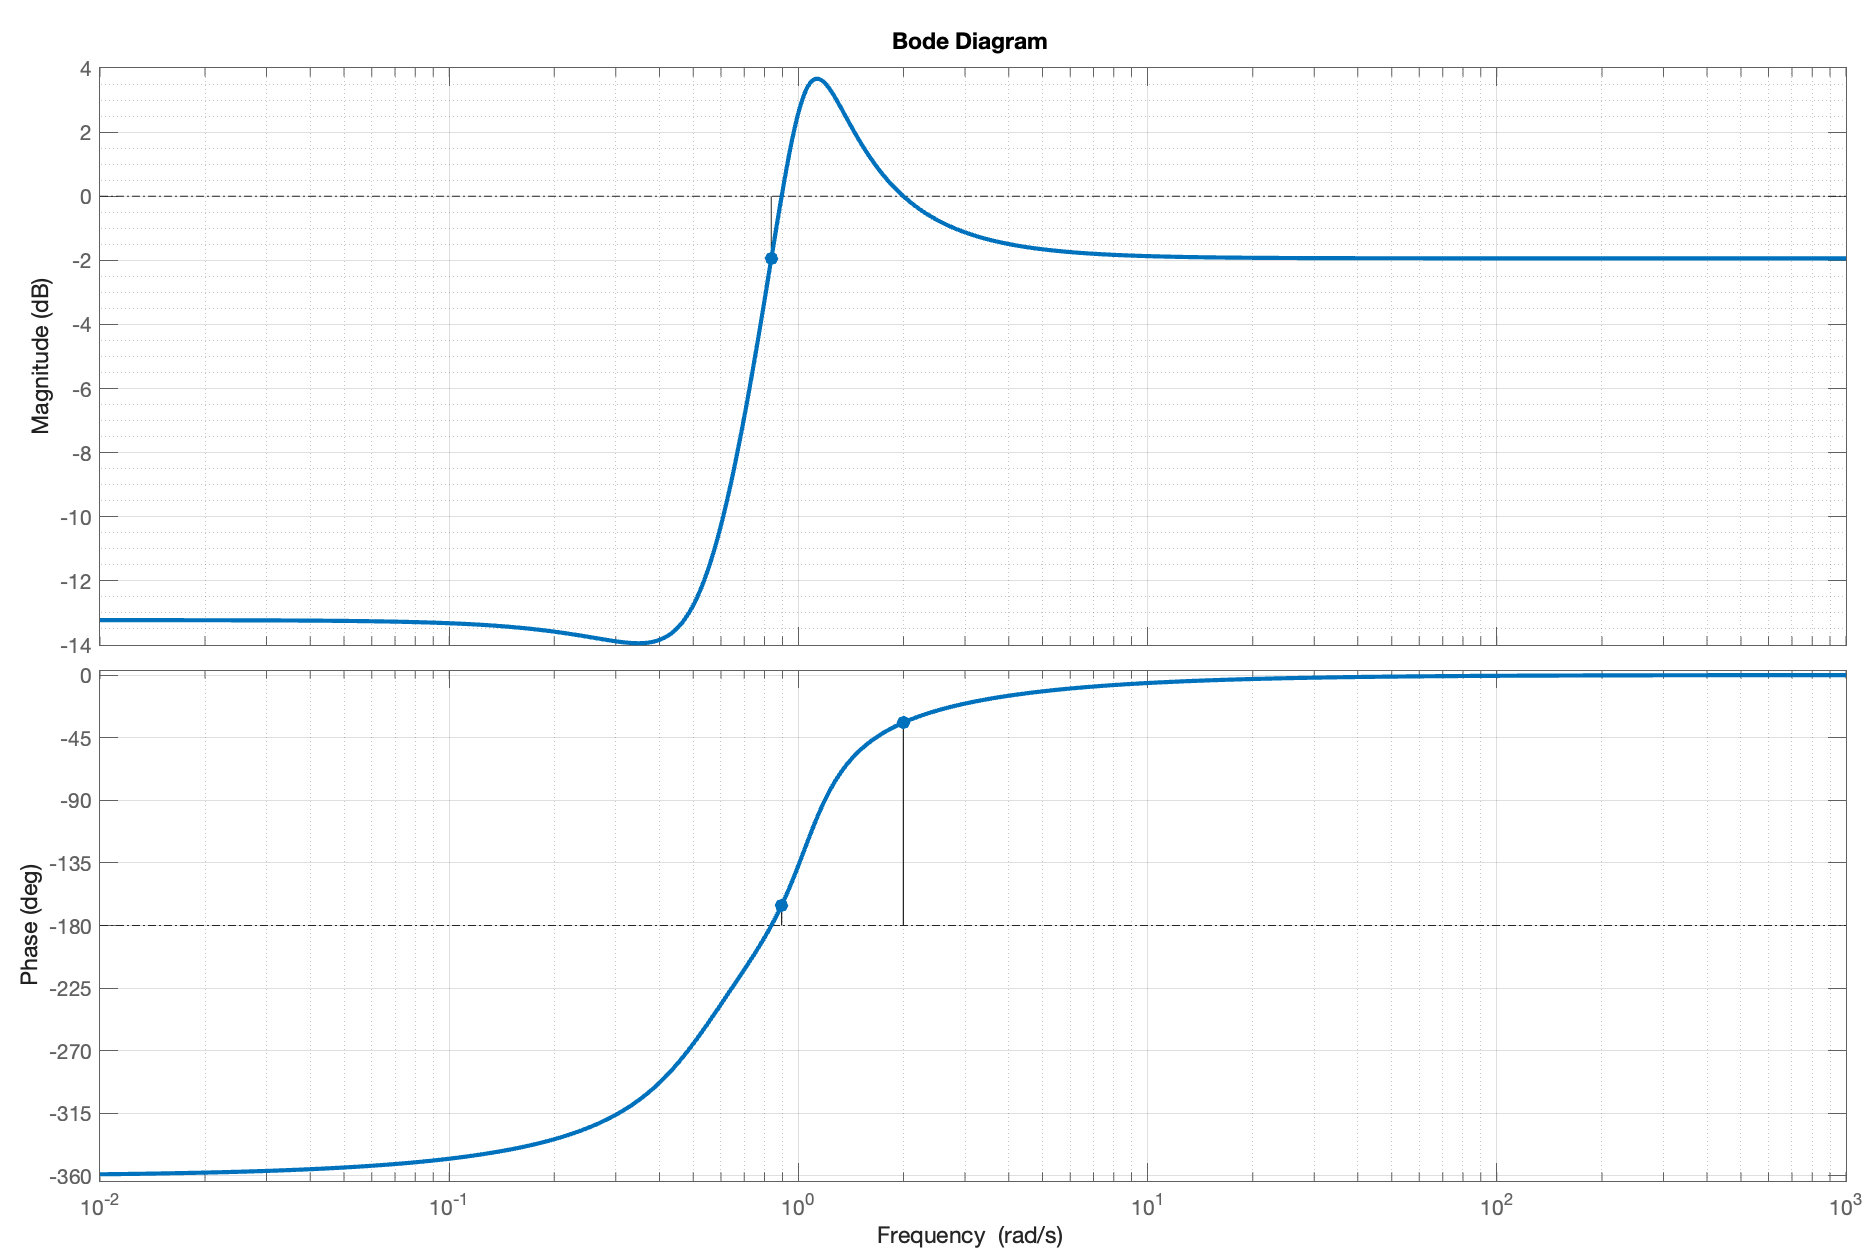
\includegraphics[width=\textwidth]{media/plots/task7_bode_open_1.png}
    \caption{ЛАФЧХ разомкнутой системы 2 при $\tau = 0$}
    \label{fig:task7_bode_open_1}
\end{figure}

Так как разомкнутая система имеет два неустойчивых полюса, нам нужно, чтобы сумма 
положительных и отрицательных переходов через критический отрезок была равна 1.
На графике видно, что нужных (при A > 0) переходов нет. Таким образом, замкнутая система будет неустойчивой.
У системы нет запаса устойчивости по фазе. 

Найдем критическое запаздывание: 
\begin{equation}
    w_{c1} = 0.89 \quad w_{c2} = 2
\end{equation}
При этом запасы по фазе будут равны $14.6^\circ = \frac{73}{900}\pi$ и $146^\circ = \frac{73}{90}\pi$ соответственно.
Найдем критические значение $\tau$: 
\begin{equation}
    \tau_{c1} = \frac{73\pi}{900 \cdot 0.89} \approx 0.29s \quad \tau_{c2} = \frac{73\pi}{90 \cdot 2} \approx 1.28s
\end{equation}
Отсюда следует, что система будет устойчива при $\tau \in (0.29, 1.28)$.

Графики переходных процессов замкнутой системы для различных значений $\tau$ представлены на рис. \ref{fig:task7_step}.
\begin{figure}[ht!]
    \begin{subfigure}{0.5\textwidth}
        \centering
        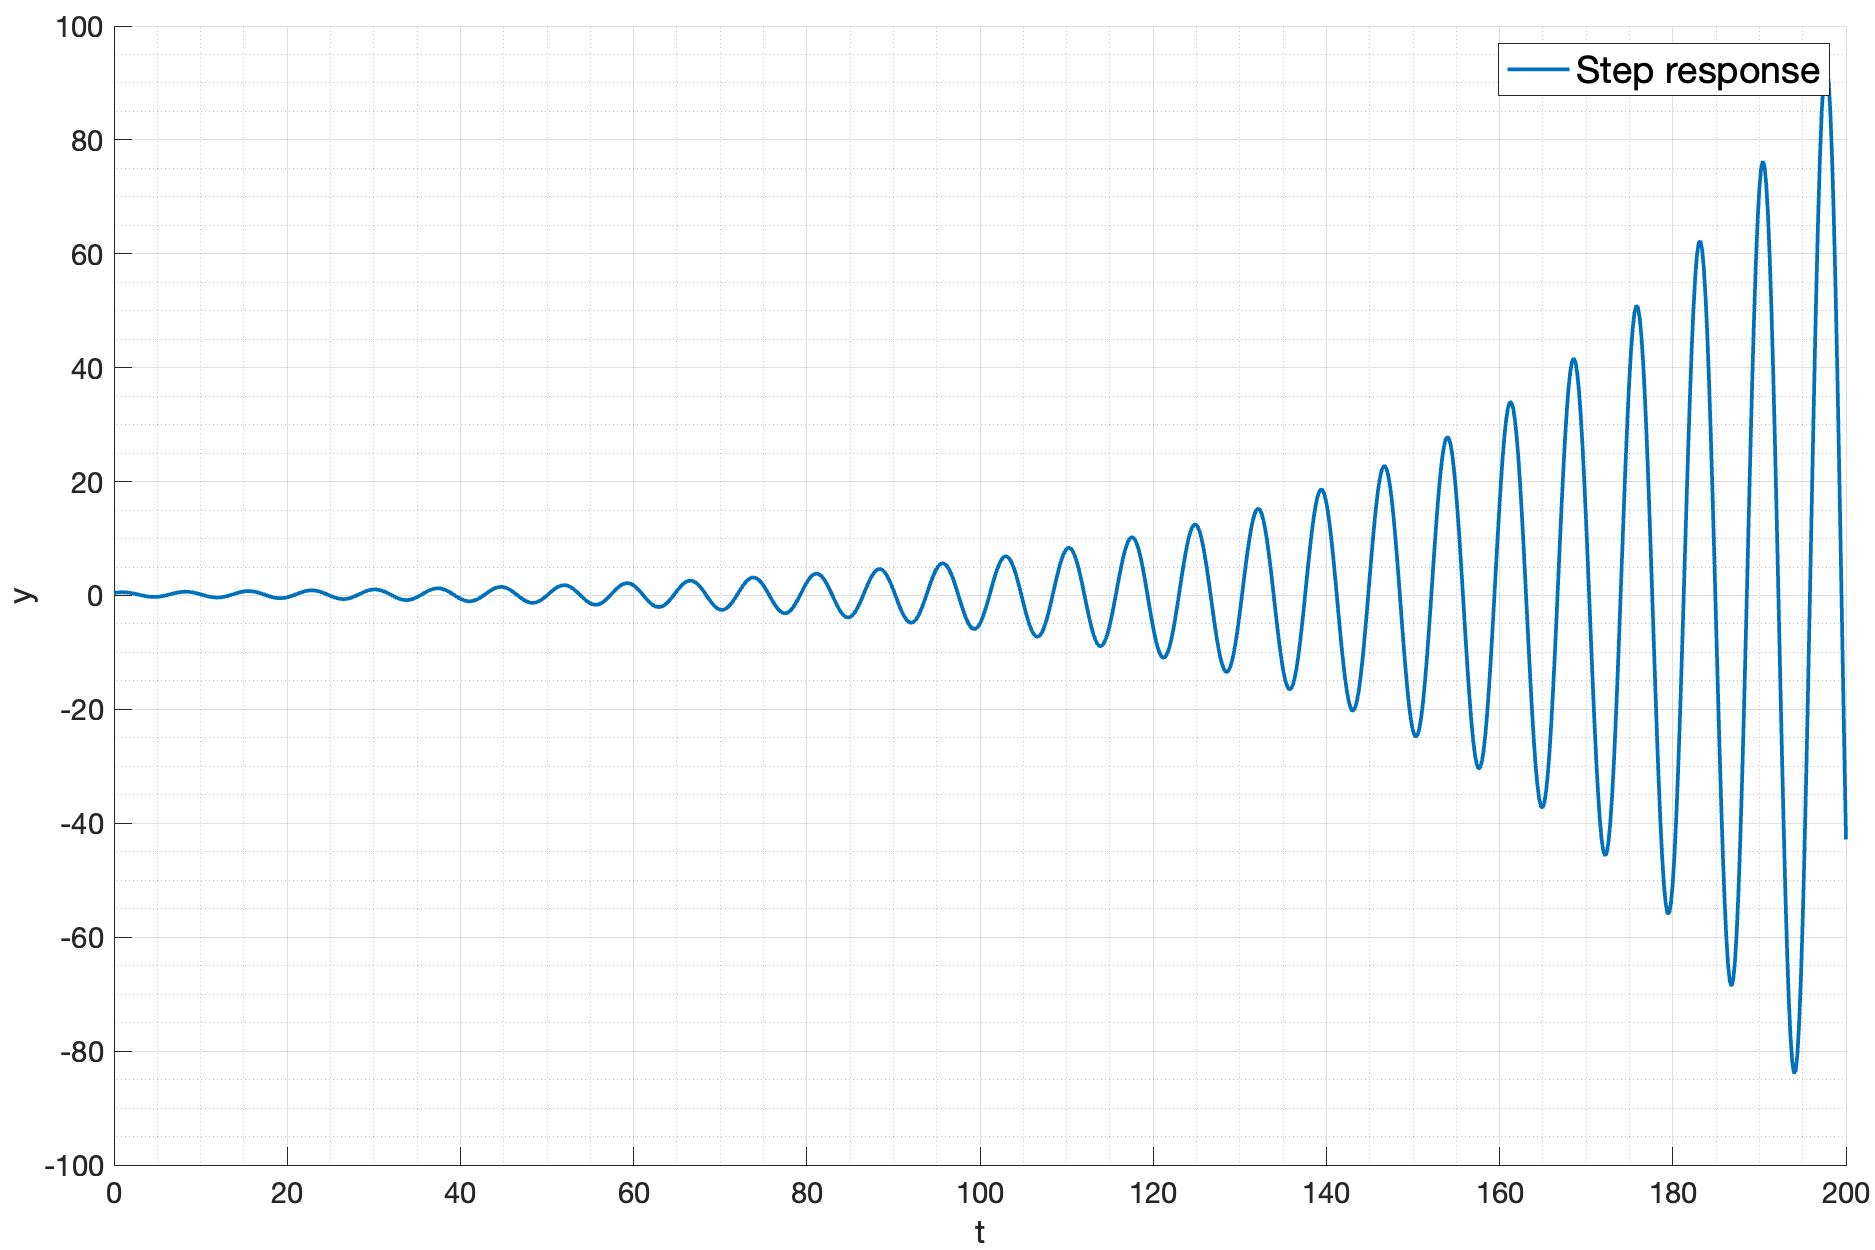
\includegraphics[width=\textwidth]{media/plots/task7_step_response_closed_1.png}
        \caption{$\tau = 0$}
    \end{subfigure}
    \begin{subfigure}{0.5\textwidth}
        \centering
        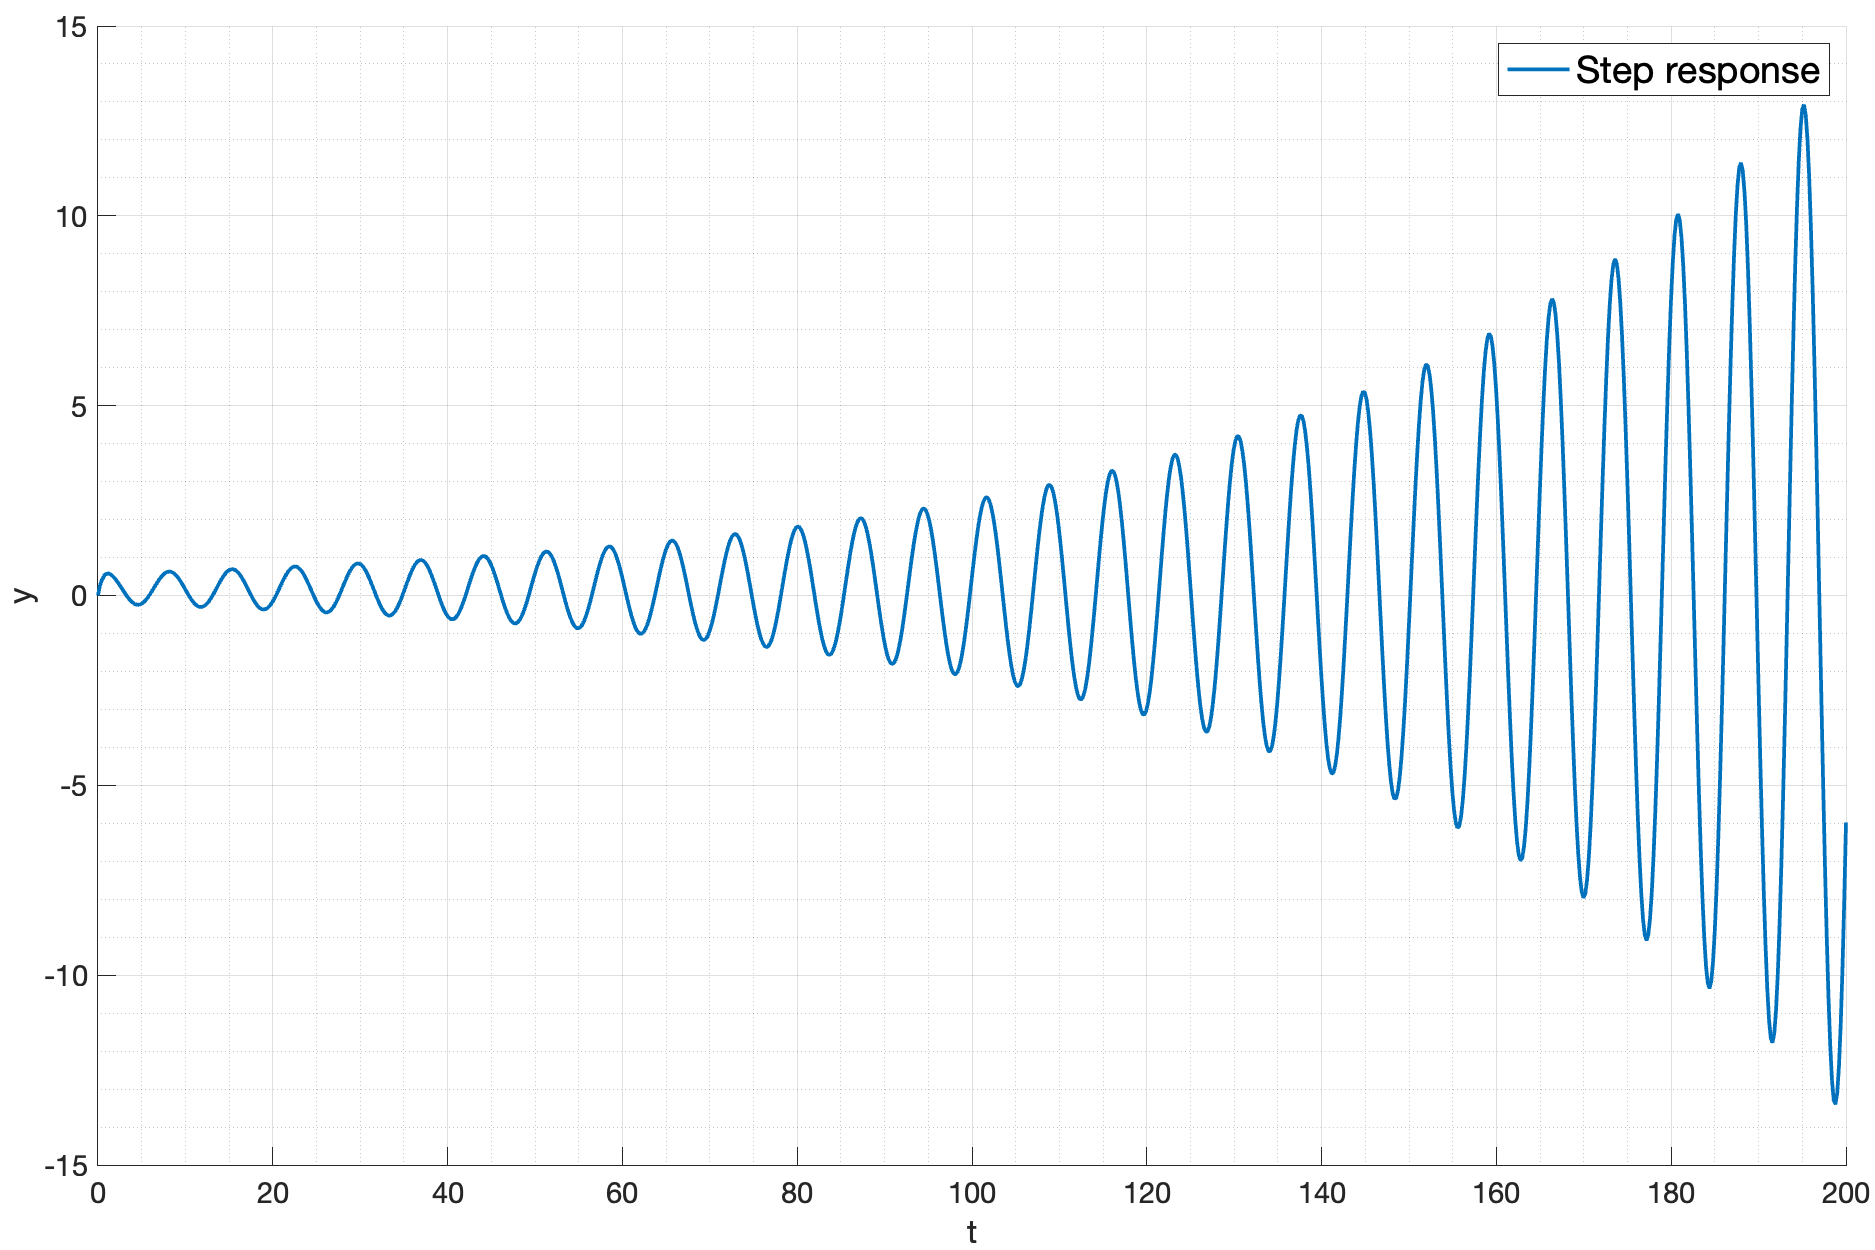
\includegraphics[width=\textwidth]{media/plots/task7_step_response_closed_2.png}
        \caption{$\tau = 0.1$}
    \end{subfigure}
    \begin{subfigure}{0.5\textwidth}
        \centering
        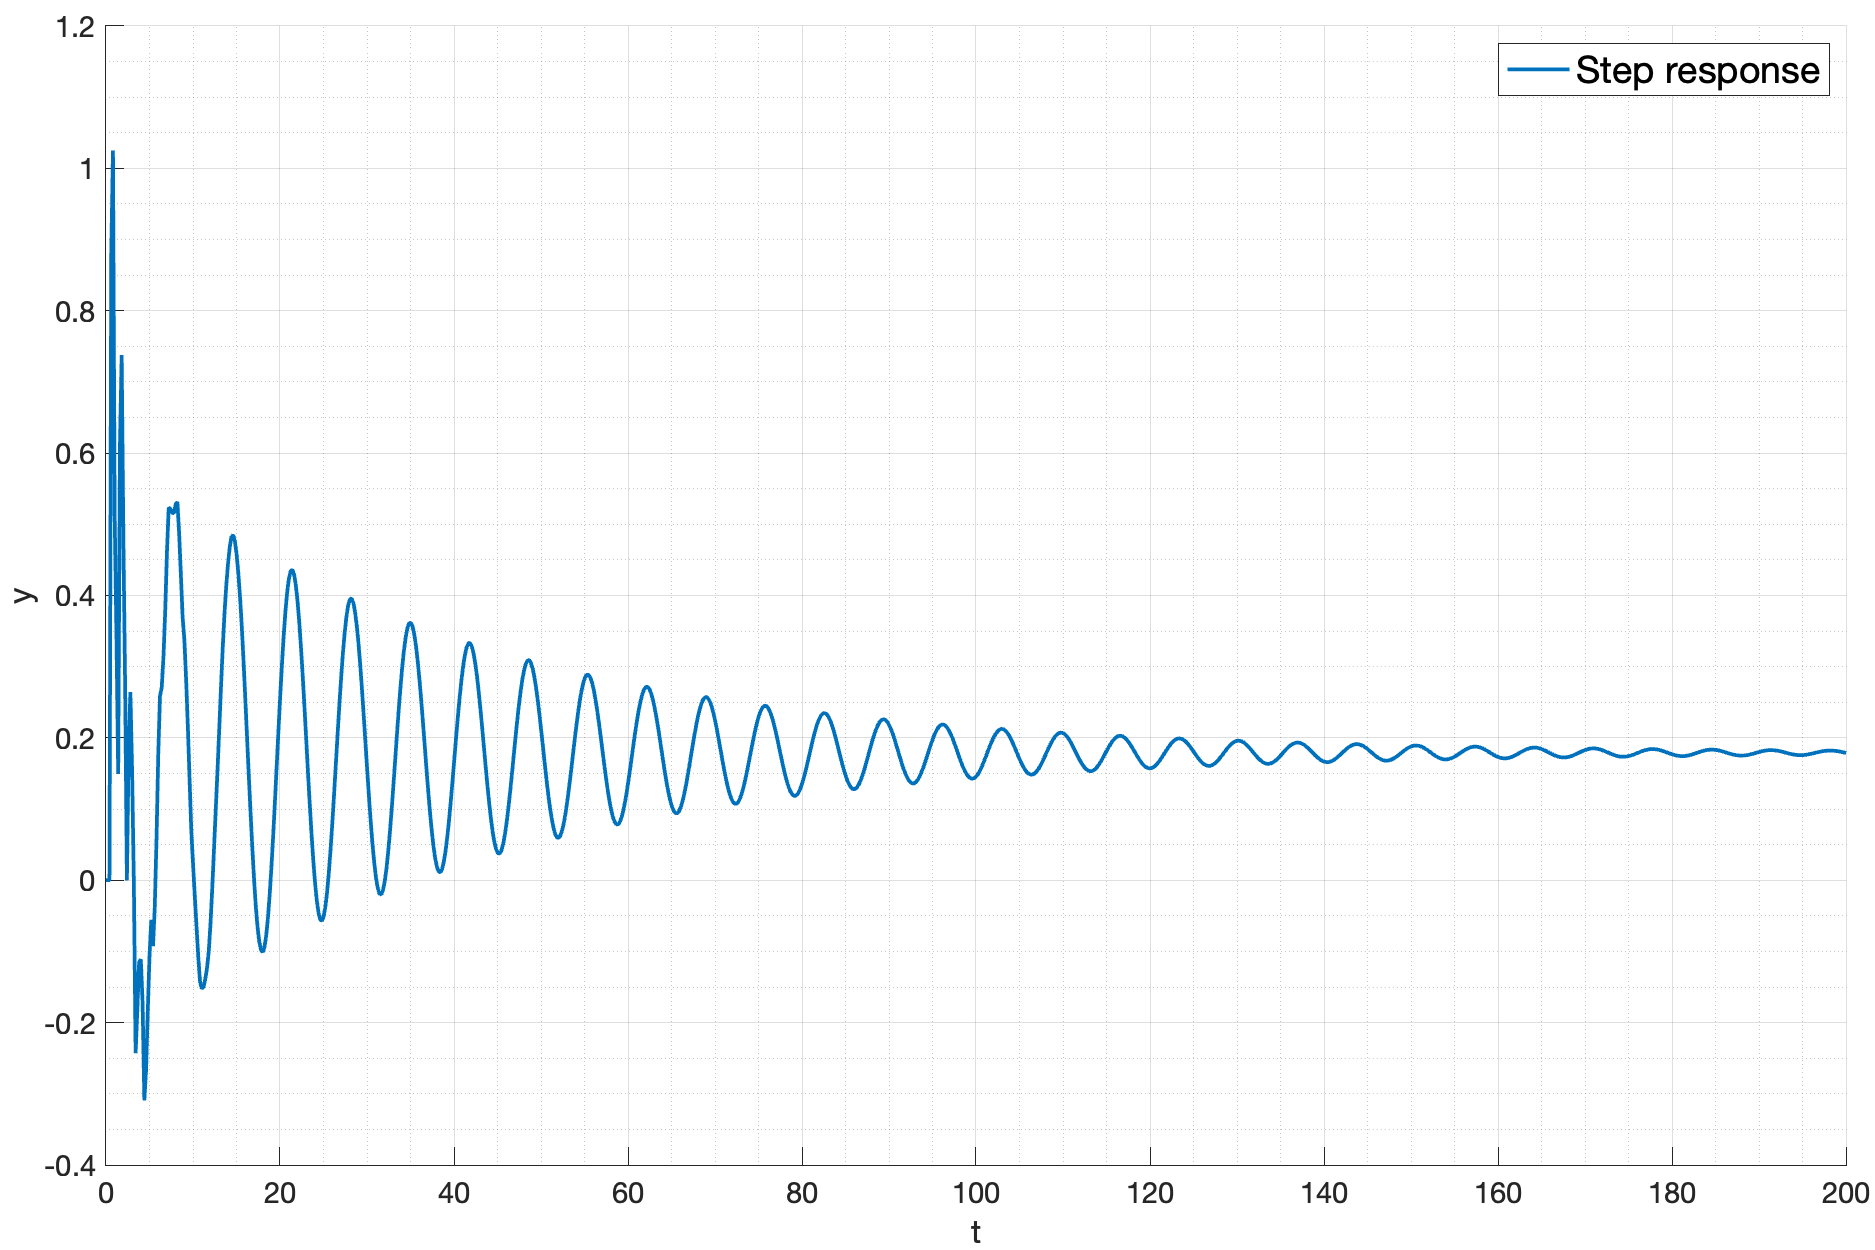
\includegraphics[width=\textwidth]{media/plots/task7_step_response_closed_3.png}
        \caption{$\tau = 0.5$}
    \end{subfigure}
    \begin{subfigure}{0.5\textwidth}
        \centering
        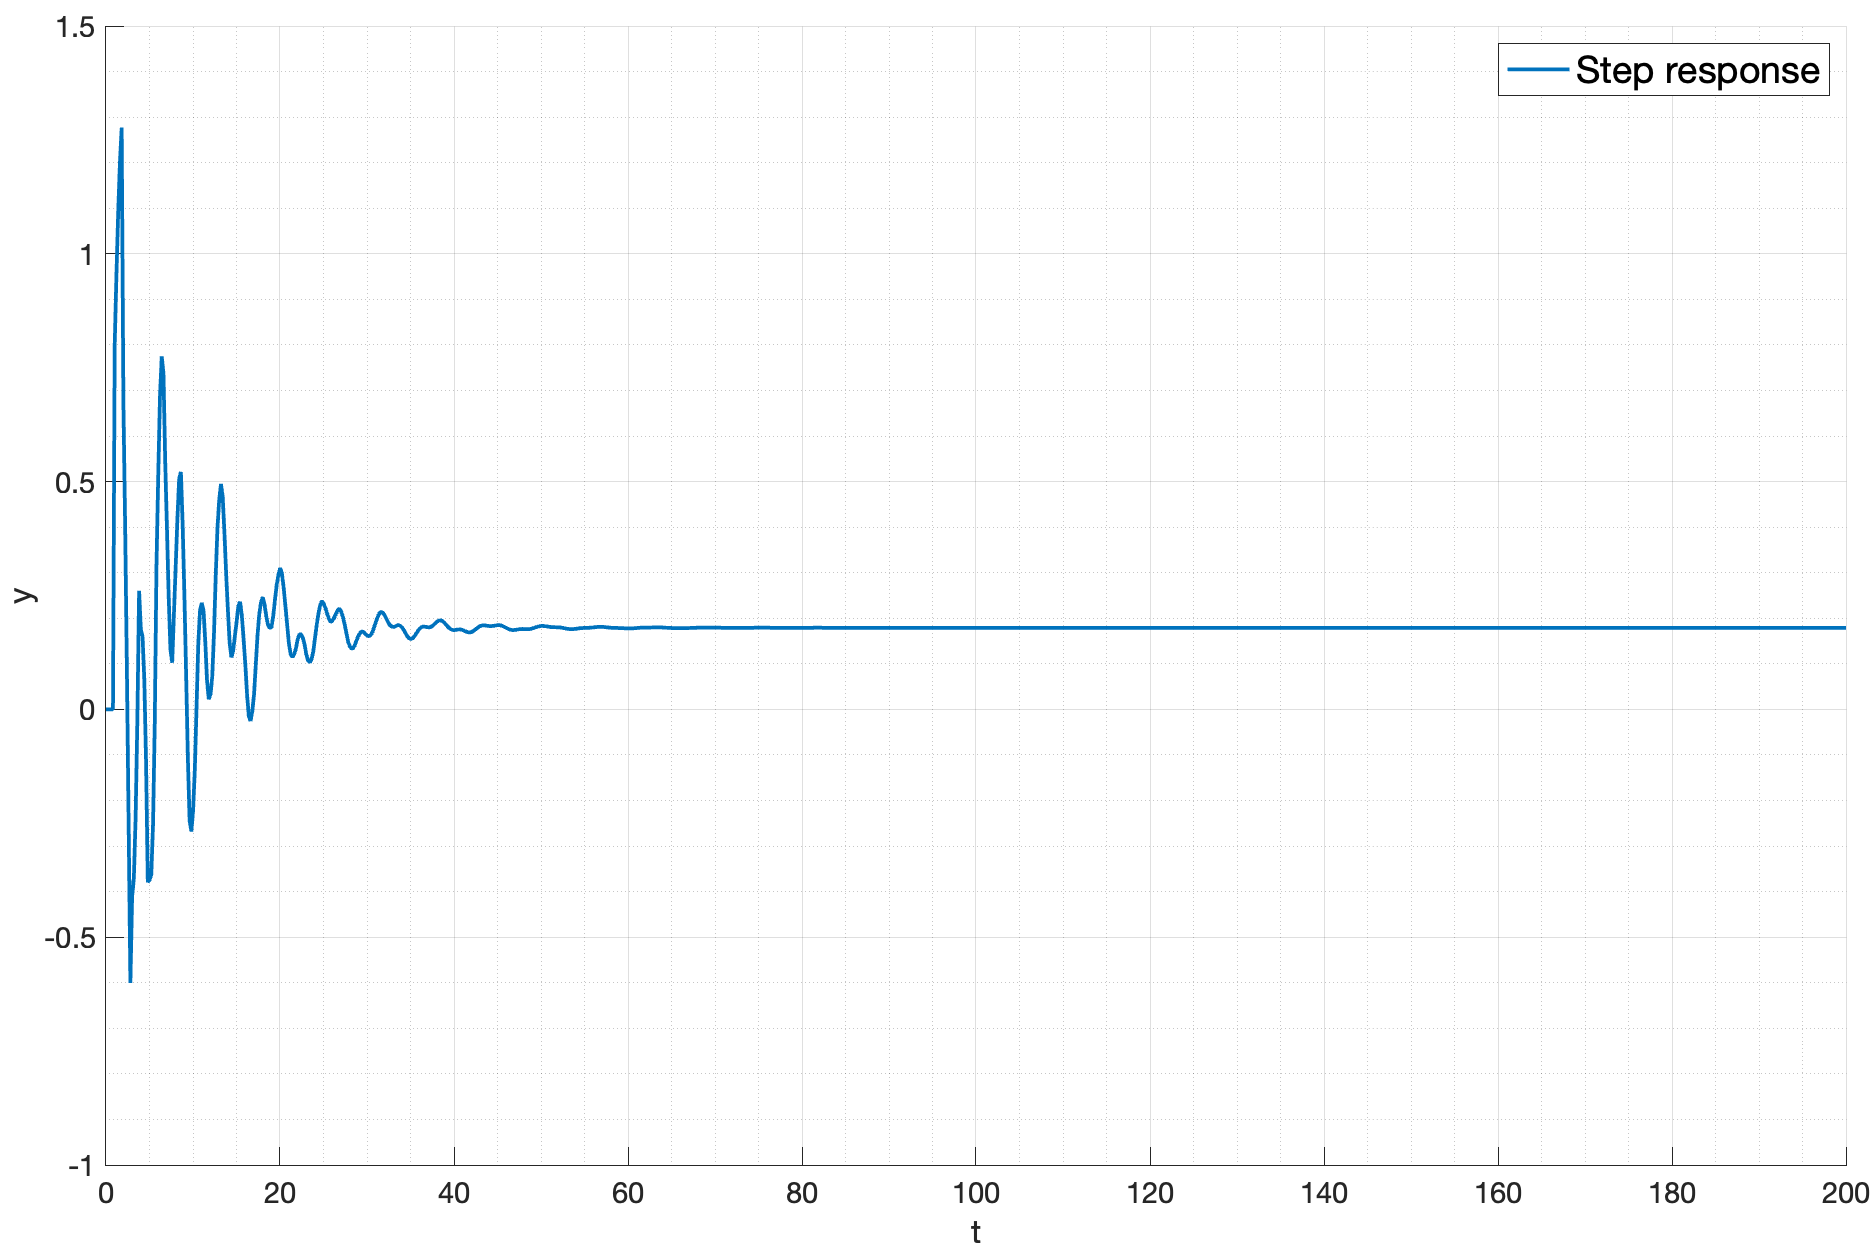
\includegraphics[width=\textwidth]{media/plots/task7_step_response_closed_4.png}
        \caption{$\tau = 1$}
    \end{subfigure}
    \begin{subfigure}{0.5\textwidth}
        \centering
        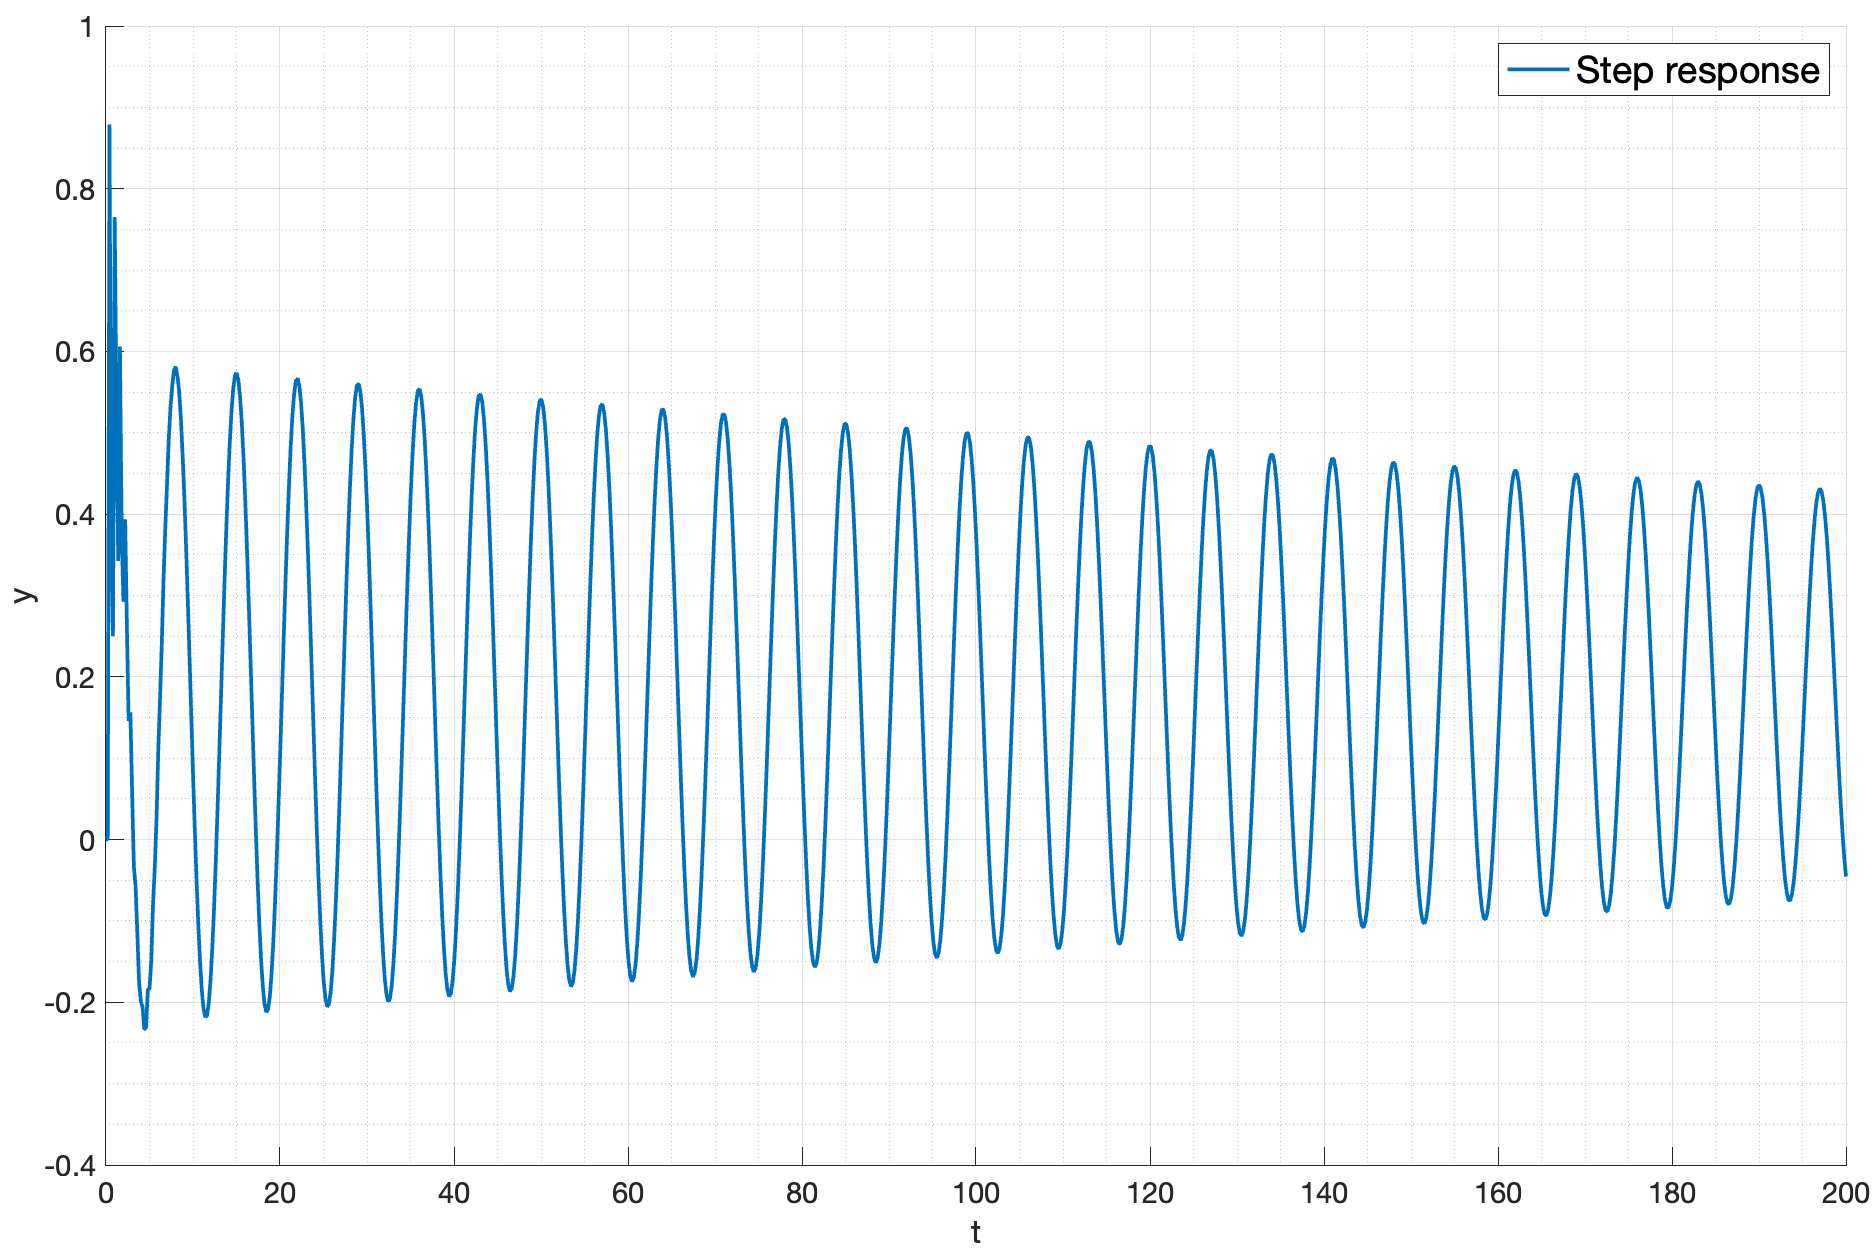
\includegraphics[width=\textwidth]{media/plots/task7_step_response_closed_5.png}
        \caption{$\tau = 0.3$}
    \end{subfigure}
    \begin{subfigure}{0.5\textwidth}
        \centering
        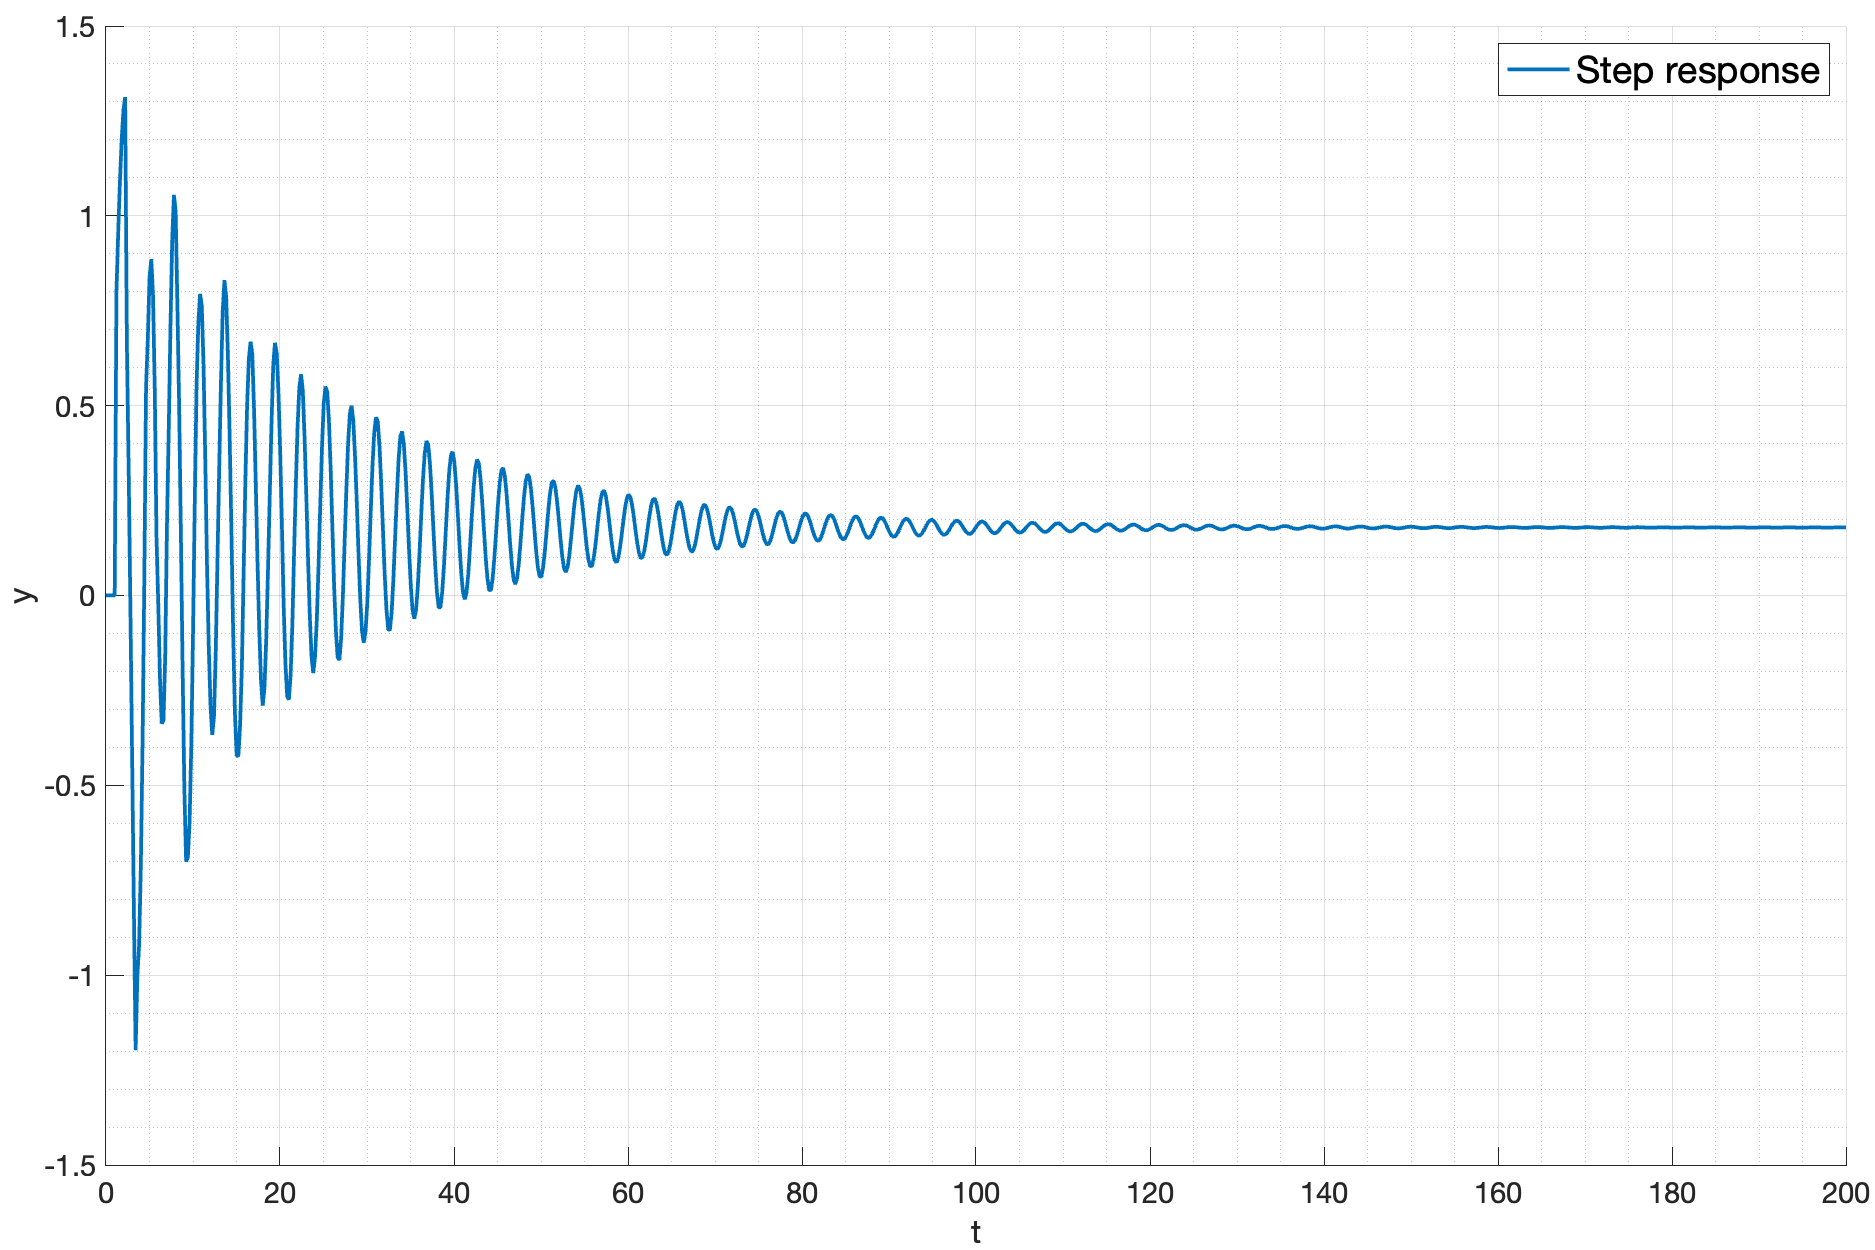
\includegraphics[width=\textwidth]{media/plots/task7_step_response_closed_6.png}
        \caption{$\tau = 1.3$}
    \end{subfigure}
    \caption{Переходные процессы для системы 2}
    \label{fig:task7_step}
\end{figure}


\subsection{Вывод}
В данном разделе были рассмотрены системы с запаздыванием. Теоретические 
рассуждения о критических значениях запаздывания подтвердились на практике, 
полученных с помощью логарифмических частотных характеристик и годографа Найквиста 
критические значения запаздывания совпали с практическими. 